% 第 6 章 增强 Qt 图形应用
\renewcommand{\codeInset}{63bp}
本章继续完善第 5 章「Qt 图形应用」中开发的三个图形 Qt 应用——模拟时钟、画图程序和编辑器。不过，我们将在本章做如下改进：

\begin{itemize}
\item 时钟：我们给钟面添加数字
\item 画图程序：增加移动和修改图形、剪切粘贴（cut-and-paste）图形以及标记一个或多个图形的能力
\item 编辑器：增加更改字体与文本对齐方式以及标记文本块的能力
\end{itemize}

本章还将继续使用 Qt 库的以下内容：

\begin{itemize}
\item 窗口与部件；
\item 菜单与工具栏；
\item 鼠标与键盘事件。
\end{itemize}

\section{改进时钟}

本章中，我们将把原来的钟面刻度线替换成数字。

\subsection{Clock 类}

Clock 类的定义与第 5 章「Qt 图形应用」中的相似。定时器每秒更新窗口 10 次。构造函数初始化时钟，每当窗口需要重绘时就会调用 paintEvent 方法。

\medskip\noindent{\ttfamily\bfseries Clock.h}

\begin{codebox}
#ifndef CLOCK_H
#define CLOCK_H

#include <QWidget>
#include <QTimer>

class Clock : public QWidget {
  Q_OBJECT

  public:
    Clock(QWidget *parentWidget = nullptr);
    void paintEvent(QPaintEvent *eventPtr);

  private:
    QTimer m_timer;
};

#endif // CLOCK_H
\end{codebox}

\medskip\noindent{\ttfamily\bfseries Clock.cpp}

\begin{codebox}
#include <QtWidgets>
#include "Clock.h"
\end{codebox}

与第 5 章「Qt 图形应用」一样，构造函数把窗口标题设置为 Clock Advanced，把窗口尺寸设置为 1000×500 像素，把定时器初始化为每 100 毫秒发送一次 timeout 消息，并把 timeout 消息连接到 update 方法——后者强制窗口在每次超时时重绘：

\begin{codebox}
Clock::Clock(QWidget *parentWidget /*= nullptr*/)
 :QWidget(parentWidget) {
  setWindowTitle(tr("Clock Advanced"));
  resize(1000, 500);

  m_timer.setParent(this);
  connect(&m_timer, SIGNAL(timeout()), this, SLOT(update()));
  m_timer.start(100);
}
\end{codebox}

每当窗口需要重绘时就会调用 paintEvent 方法。我们首先计算时钟的边长，并获取当前时间：

\begin{codebox}
void Clock::paintEvent(QPaintEvent* /*event*/) {
  int side = qMin(width(), height());
  QTime time = QTime::currentTime();
\end{codebox}

接着，我们创建并初始化一个 QPainter 对象。我们调用 translate 和 scale，把物理尺寸（像素）匹配到 200×200 单位的逻辑尺寸：

\begin{codebox}
  QPainter painter(this);
  painter.setRenderHint(QPainter::Antialiasing);
  painter.setRenderHint(QPainter::TextAntialiasing);
  painter.translate(width() / 2, height() / 2);
  painter.scale(side / 200.0, side / 200.0);
\end{codebox}

由于本版的时钟要在钟面上书写数字，我们为画笔添加 12 磅的 Times New Roman 字体：

\begin{codebox}
  painter.setFont(QFont(tr("Times New Roman"), 12));
\end{codebox}

我们把时钟的数字 1 到 12 写在钟面上，如下面的代码所示：

\begin{codebox}
  for (int hour = 1; hour <= 12; ++hour) {
    QString text;
    text.setNum(hour);
\end{codebox}

一整圈是 $360^\circ$，相邻两个数字之间的夹角是 $30^\circ$，因为 360 除以 12 等于 30：

\begin{codebox}
  double angle = (30.0 * hour) - 90;
  double radius = 90.0;
\end{codebox}

数字的 x 和 y 坐标由正弦函数和余弦函数计算。不过，我们首先要把角度换算成弧度，因为正弦和余弦只接受弧度。如下面的代码所示：

\begin{codebox}
  double x = radius * qCos(qDegreesToRadians(angle)),
         y = radius * qSin(qDegreesToRadians(angle));
\end{codebox}

drawText 方法写出数字，如下所示：

\begin{codebox}
  QRect rect(x - 100, y - 100, 200, 200);
  painter.drawText(rect, Qt::AlignHCenter |
                        Qt::AlignVCenter, text);
  }
\end{codebox}

数字写完之后，我们按照与第 5 章「Qt 图形应用」相同的方式绘制时针、分针和秒针：

\begin{codebox}
  double hours = time.hour(), minutes = time.minute(),
    seconds = time.second(), milliseconds = time.msec();

  painter.setPen(Qt::black);
  painter.setBrush(Qt::gray);

  { static const QPoint hourHand[3] =
     {QPoint(8, 8), QPoint(-8, 8), QPoint(0, -60)};

    painter.save();
    double hour = hours + (minutes / 60.0) + (seconds / 3600.0) +
                 (milliseconds / 3600000.0);
    painter.rotate(30.0 * hour);
    painter.drawConvexPolygon(hourHand, 3);
    painter.restore();
  }

  { static const QPoint minuteHand[3] =
    {QPoint(6, 8), QPoint(-6, 8), QPoint(0, -70)};

    painter.save();
    double minute = minutes + (seconds / 60.0) +
                   (milliseconds / 60000.0);
    painter.rotate(6.0 * minute);
    painter.drawConvexPolygon(minuteHand, 3);
    painter.restore();
  }

  { static const QPoint secondHand[3] =
     {QPoint(4, 8), QPoint(-4, 8), QPoint(0, -80)};

    painter.save();
    double second = seconds + (milliseconds / 1000);
    painter.rotate(6.0 * second);
    painter.drawConvexPolygon(secondHand, 3);
    painter.restore();
  }
}
\end{codebox}

\subsection{main 函数}

main 函数与第 5 章「Qt 图形应用」中的相似。它创建应用对象，初始化时钟，然后执行应用。

\medskip\noindent{\ttfamily\bfseries Main.cpp}

\begin{codebox}
#include <QApplication>
#include "Clock.h"

int main(int argc, char *argv[]) {
  QApplication application(argc, argv);
  Clock Clock;
  Clock.show();
  return application.exec();
}
\end{codebox}

程序的输出如下面的截图所示：

\begin{center}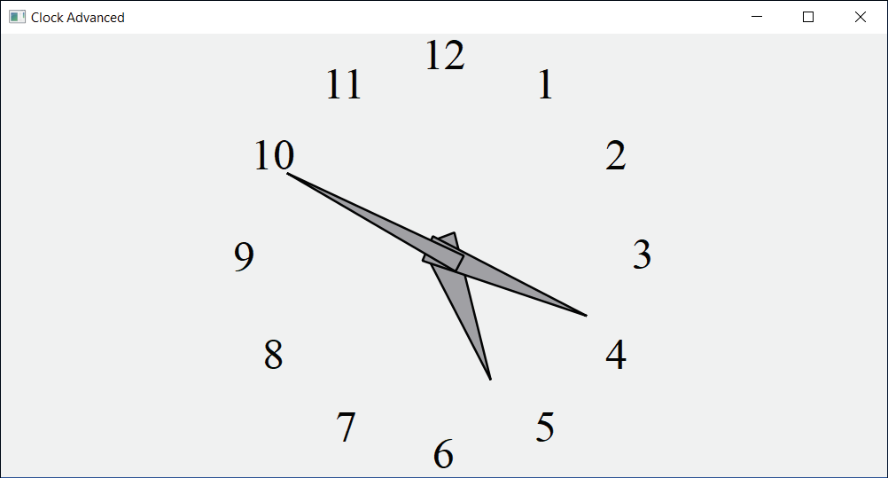
\includegraphics[width=0.9\textwidth]{images/p245_i08.png}\end{center}

\section{改进画图程序}

本章的画图程序是第 5 章「Qt 图形应用」中画图程序的高级版本。在这一版本中，我们可以修改图形，可以圈选一个或多个图形然后更改它们的颜色，还可以剪切粘贴图形。

\subsection{Figure 类}

Figure 类与第 5 章「Qt 图形应用」中的相当相似，不过新增了 isInside、doubleClick、modify 和 marked。

\medskip\noindent{\ttfamily\bfseries Figure.h}

\begin{codebox}
#ifndef FIGURE_H
#define FIGURE_H

enum FigureId {LineId, RectangleId, EllipseId};

#include <QtWidgets>
#include <FStream>
using namespace std;

class Figure {
  public:
  Figure();
\end{codebox}

本版新增了纯虚函数 clone，这是为了支持剪切粘贴。粘贴图形时，我们想创建它的副本，而实际上并不知道该对象属于哪个类。仅靠复制构造函数无法做到这一点。这正是本节的核心：如何使用纯虚方法，以及如何利用动态绑定。我们需要 clone，它调用所属类的复制构造函数，返回指向新对象的指针：

\begin{codebox}
  virtual Figure* clone() const = 0;

  virtual FigureId getId() const = 0;
  virtual void initializePoints(QPoint point) = 0;
\end{codebox}

在本版的画图程序中，onClick 会设置一些字段，指明图形应被修改还是被移动。如果用户抓取了图形的某个抓取点（不同种类的图形各不相同），就修改图形；否则就移动图形。当用户抓取图形的某个角时调用 modify 方法。此时图形将被修改而不是移动：

\begin{codebox}
  virtual bool isClick(QPoint mousePoint) = 0;
  virtual void modify(QSize distance) = 0;
\end{codebox}

如果图形完全被圈在区域内，isInside 方法就返回 true。当用户用鼠标圈选图形时会调用它：

\begin{codebox}
  virtual bool isInside(QRect area) = 0;
\end{codebox}

当用户在图形上双击时调用 doubleClick 方法，每种图形会执行某个合适的动作：

\begin{codebox}
  virtual void doubleClick(QPoint mousePoint) = 0;
  virtual void move(QSize distance) = 0;
  virtual void draw(QPainter &painter) const = 0;
  virtual bool write(ofstream& outStream) const;
  virtual bool read(ifstream& inStream);
\end{codebox}

marked 方法返回并设置 \texttt{m\_marked} 字段。图形被标记之后，会用一些小方块标注出来：

\begin{codebox}
  bool marked() const {return m_marked;}
  bool& marked() {return m_marked;}

  const QColor& color() const {return m_color;}
  QColor& color() {return m_color;}

  virtual bool filled() const {return m_filled;}
  virtual bool& filled() {return m_filled;}

  static const int Tolerance;

  private:
    QColor m_color;
    bool m_marked = false, m_filled = false;
};

#endif
\end{codebox}

\medskip\noindent{\ttfamily\bfseries Figure.cpp}

\begin{codebox}
#include "..\MainWindow\DocumentWidget.h"
#include "Figure.h"

const int Figure::Tolerance(6);

Figure::Figure() {
   // Empty.
}
\end{codebox}

write 和 read 方法写出并读取图形的颜色以及是否填充。不过，它们不写出也不读取标记状态。图形在写出或读取时总是处于未标记状态：

\begin{codebox}
bool Figure::write(ofstream& outStream) const {
  writeColor(outStream, m_color);
  outStream.write((char*) &m_filled, sizeof m_filled);
  return ((bool) outStream);
}

bool Figure::read(ifstream& inStream) {
  readColor(inStream, m_color);
  inStream.read((char*) &m_filled, sizeof m_filled);
  return ((bool) inStream);
}
\end{codebox}

\subsection{Line 类}

Line 类是 Figure 的子类。

\medskip\noindent{\ttfamily\bfseries Line.h}

\begin{codebox}
#ifndef LINE_H
#define LINE_H

#include <FStream>
using namespace std;

#include "Figure.h"

class Line : public Figure {
  public:
  Line();
  FigureId getId() const {return LineId;}
  Line(const Line& line);
  Figure* clone() const;
  void initializePoints(QPoint point);
\end{codebox}

正如前面 Figure 节提到的，isClick 决定直线应被修改还是被移动。如果用户抓取了直线的某个端点，就只移动该端点。如果用户抓取了两个端点之间的直线，就移动整条直线。也就是说，直线的两个端点都要移动：

\begin{codebox}
  bool isClick(QPoint mousePoint);
\end{codebox}

isInside 方法检查直线是否完全被区域圈住：

\begin{codebox}
  bool isInside(QRect area);
\end{codebox}

doubleClick 方法在 Line 类中什么也不做。不过，我们仍然需要定义它，因为它在 Figure 中是纯虚的。如果不定义它，Line 就会变成抽象类：

\begin{codebox}
  void doubleClick(QPoint /* mousePoint */) {/* Empty. */}
\end{codebox}

modify 方法按照前面的 isClick 所做的设置来修改直线。如果用户抓取了某个端点，就移动该端点；否则移动整条直线（两个端点都移动）：

\begin{codebox}
  void modify(QSize distance);
  void move(QSize distance);
\end{codebox}

如果直线被标记，area 方法就返回一个稍微扩大了的区域，以便把标记方块包含进来：

\begin{codebox}
  QRect area() const;
  void draw(QPainter& painter) const;
  bool write(ofstream& outStream) const;
  bool read(ifstream& inStream);
\end{codebox}

\texttt{m\_lineMode} 字段记录直线的移动或修改状态。直线创建时，\texttt{m\_lineMode} 被设置为 LastPoint。当用户抓取直线的第一个或最后一个端点时，\texttt{m\_lineMode} 被设置为 FirstPoint 或 LastPoint。当用户抓取两个端点之间的直线时，\texttt{m\_lineMode} 被设置为 MoveLine：

\begin{codebox}
  private:
       enum {FirstPoint, LastPoint, MoveLine} m_lineMode;
       QPoint m_firstPoint, m_lastPoint;
\end{codebox}

isPointInLine 方法判断用户是否在一定的容差范围内点击了直线：

\begin{codebox}
  static bool isPointInLine(QPoint m_firstPoint,
                            QPoint m_lastPoint, QPoint point);
};

#endif
\end{codebox}

\medskip\noindent{\ttfamily\bfseries Line.cpp}

\begin{codebox}
#include "..\MainWindow\DocumentWidget.h"
#include "Line.h"
\end{codebox}

直线创建时，直线模式被设置为最后一个端点。也就是说，用户移动鼠标时，改变的是直线的最后一个端点：

\begin{codebox}
Line::Line()
:m_lineMode(LastPoint) {
  // Empty.
}
\end{codebox}

粘贴直线时会调用 clone 方法。这里调用 Figure 的复制构造函数来设置图形的颜色。注意，我们以一个 Line 对象为参数调用 Figure 构造函数，尽管它接受的是一个 Figure 对象的引用。这样做是允许的，因为 Line 是 Figure 的子类，调用期间 Line 对象会被转换成 Figure 对象。此外，直线的第一个和最后一个端点也被复制。注意，我们不需要复制 \texttt{m\_lineMode} 的值，因为它只在用户创建、修改或移动直线时才会被设置：

\begin{codebox}
Line::Line(const Line& line)
 :Figure(line),
   m_firstPoint(line.m_firstPoint),
   m_lastPoint(line.m_lastPoint) {
  // Empty.
 }
\end{codebox}

clone 方法用复制构造函数创建一个新对象，然后把它返回：

\begin{codebox}
Figure* Line::clone() const {
  Line* linePtr = new Line(*this);
  return linePtr;
}
\end{codebox}

直线创建之后不久会调用 initializePoints 方法。之所以有这一步，是因为我们并不直接创建 Line 对象，而是通过调用 clone 间接创建直线。因此，我们需要调用 initializePoints 来初始化两个端点：

\begin{codebox}
void Line::initializePoints(QPoint point) {
  m_firstPoint = point;
  m_lastPoint = point;
}
\end{codebox}

用户用鼠标点击时会调用 isClick 方法。我们首先检查用户是否点击了第一个端点。我们利用 Tolerance 字段创建一个小方块，以第一个端点为中心。如果用户点击了这个方块，就把 \texttt{m\_lineMode} 设置为 FirstPoint 并返回 true：

\begin{codebox}
bool Line::isClick(QPoint mousePoint) {
  QRect firstSquare(makeRect(m_firstPoint, Tolerance));

  if (firstSquare.contains(mousePoint)) {
   m_lineMode = FirstPoint;
   return true;
 }
\end{codebox}

以同样的方式，我们创建一个以最后一个端点为中心的小方块。如果用户点击了这个方块，就把 \texttt{m\_lineMode} 设置为 LastPoint 并返回 true：

\begin{codebox}
  QRect lastSquare(makeRect(m_lastPoint, Tolerance));

  if (lastSquare.contains(mousePoint)) {
    m_lineMode = LastPoint;
    return true;
  }
\end{codebox}

如果用户没有点击任何一个端点，我们就检查用户是否点击了直线本身。如果是，就把 \texttt{m\_lineMode} 设置为 MoveLine 并返回 true：

\begin{codebox}
  if (isPointInLine(m_firstPoint, m_lastPoint, mousePoint)) {
    m_lineMode = MoveLine;
    return true;
  }
\end{codebox}

最后，如果用户既没有点击端点也没有点击直线本身，就说明完全没点到这条直线，返回 false：

\begin{codebox}
  return false;
}
\end{codebox}

如果直线完全被区域圈住，isInside 方法就返回 true。这很容易：我们只需检查两个端点是否都位于区域内：

\begin{codebox}
bool Line::isInside(QRect area) {
 return area.contains(m_firstPoint) &&
   area.contains(m_lastPoint);
}
\end{codebox}

isPointInLine 方法与第 5 章「Qt 图形应用」版本中的 isClick 完全相同：

\begin{codebox}
bool Line::isPointInLine(QPoint m_firstPoint, QPoint m_lastPoint,
                         QPoint point) {
  if (m_firstPoint.x() == m_lastPoint.x()) {
    QRect lineRect(m_firstPoint, m_lastPoint);
    lineRect.normalized();
    lineRect += Tolerance;
    return lineRect.contains(point);
  }
  else {
    QPoint leftPoint = (m_firstPoint.x() < m_lastPoint.x())
                       ? m_firstPoint : m_lastPoint,
           rightPoint = (m_firstPoint.x() < m_lastPoint.x())
                        ? m_lastPoint : m_firstPoint;

    if ((leftPoint.x() <= point.x()) &&
        (point.x() <= rightPoint.x())) {
      int lineWidth = rightPoint.x() - leftPoint.x(),
          lineHeight = rightPoint.y() - leftPoint.y();

      int diffWidth = point.x() - leftPoint.x(),
          diffHeight = point.y() - leftPoint.y();

      double delta = fabs(diffHeight -
               (diffWidth * ((double) lineHeight) / lineWidth));

      return (delta <= Tolerance);
    }

    return false;
  }
}
\end{codebox}

modify 方法根据前面的 isClick 方法中对 \texttt{m\_lineMode} 的设置，移动第一个端点、最后一个端点，或者两个端点：

\begin{codebox}
void Line::modify(QSize distance) {
  switch (m_lineMode) {
    case FirstPoint:
    m_firstPoint += distance;
    break;

    case LastPoint:
    m_lastPoint += distance;
    break;

    case MoveLine:
    move(distance);
    break;
  }
}
\end{codebox}

move 方法只是把直线的两个端点都移动一下：

\begin{codebox}
void Line::move(QSize distance) {
  m_firstPoint += distance;
  m_lastPoint += distance;
}
\end{codebox}

draw 方法绘制直线。与第 5 章「Qt 图形应用」的版本相比，不同之处在于：如果直线被标记，还会在直线两端绘制方块：

\begin{codebox}
void Line::draw(QPainter& painter) const {
  painter.setPen(color());
  painter.drawLine(m_firstPoint, m_lastPoint);

  if (marked()) {
    painter.fillRect(makeRect(m_firstPoint, Tolerance),
                     Qt::black);
    painter.fillRect(makeRect(m_lastPoint, Tolerance),
                     Qt::black);
  }
}
\end{codebox}

area 方法返回覆盖直线的区域。如果直线被标记，区域会稍微扩大，以便覆盖标记端点的方块：

\begin{codebox}
QRect Line::area() const {
  QRect lineArea(m_firstPoint, m_lastPoint);
  lineArea.normalized();

  if (marked()) {
     lineArea += Tolerance;
  }

  return lineArea;
}
\end{codebox}

与第 5 章「Qt 图形应用」的版本一样，write 和 read 先调用 Figure 中的对应方法，然后写出并读取直线的两个端点：

\begin{codebox}
bool Line::write(ofstream& outStream) const {
  Figure::write(outStream);
  writePoint(outStream, m_firstPoint);
  writePoint(outStream, m_lastPoint);
  return ((bool) outStream);
}

bool Line::read(ifstream& inStream) {
  Figure::read(inStream);
  readPoint(inStream, m_firstPoint);
  readPoint(inStream, m_lastPoint);
  return ((bool) inStream);
}
\end{codebox}

\subsection{Rectangle 类}

RectangleX 是 Figure 的子类，是第 5 章「Qt 图形应用」版本的扩展版本。其中 isClick 方法经过了修改，还新增了 doubleClick 和 modify。

\medskip\noindent{\ttfamily\bfseries Rectangle.h}

\begin{codebox}
#ifndef RECTANGLE_H
#define RECTANGLE_H

#include <FStream>
using namespace std;

#include "Figure.h"

class RectangleX : public Figure {
  public:
  RectangleX();
  virtual FigureId getId() const {return RectangleId;}

  RectangleX(const RectangleX& rectangle);
  Figure* clone() const;

  virtual void initializePoints(QPoint point);

  virtual bool isClick(QPoint mousePoint);
  virtual void modify(QSize distance);
  virtual bool isInside(QRect area);
  virtual void doubleClick(QPoint mousePoint);

  virtual void move(QSize distance);
  virtual QRect area() const;
  virtual void draw(QPainter& painter) const;

  virtual bool write(ofstream& outStream) const;
  virtual bool read(ifstream& inStream);

  private:
    enum {TopLeftPoint, TopRightPoint, BottomRightPoint,
        BottomLeftPoint, MoveRectangle} m_rectangleMode;

  protected:
    QPoint m_topLeft, m_bottomRight;
};

#endif
\end{codebox}

\medskip\noindent{\ttfamily\bfseries Rectangle.cpp}

\begin{codebox}
#include <CAssert>
#include "..\MainWindow\DocumentWidget.h"
#include "Rectangle.h"
\end{codebox}

用户添加矩形时，其模式为 BottomRightPoint。也就是说，用户移动鼠标时，改变的是矩形的右下角：

\begin{codebox}
RectangleX::RectangleX()
:m_rectangleMode(BottomRightPoint) {
  // Empty.
}
\end{codebox}

复制构造函数复制矩形。具体来说，它先调用 Figure 类的复制构造函数，然后复制左上角和右下角。注意，它不复制 \texttt{m\_rectangleMode} 字段，因为这个字段只在用户移动鼠标时才会用到：

\begin{codebox}
RectangleX::RectangleX(const RectangleX& rectangle)
:Figure(rectangle),
  m_topLeft(rectangle.m_topLeft),
  m_bottomRight(rectangle.m_bottomRight) {
  // Empty.
}
\end{codebox}

clone 方法调用复制构造函数来创建一个新对象，并返回指向它的指针：

\begin{codebox}
Figure* RectangleX::clone() const {
  RectangleX* rectanglePtr = new RectangleX(*this);
  return rectanglePtr;
}

void RectangleX::initializePoints(QPoint point) {
  m_topLeft = point;
  m_bottomRight = point;
}
\end{codebox}

用户用鼠标点击时会调用 isClick 方法。与前面的 Line 类似，我们首先检查用户是否点击了任意一个角。如果没有，再根据矩形是否为填充状态，检查用户点击的是矩形边框还是矩形内部。

我们先定义一个覆盖左上角的小方块。如果用户点击了它，就把 \texttt{m\_rectangleMode} 字段设置为 TopLeftPoint 并返回 true：

\begin{codebox}
bool RectangleX::isClick(QPoint mousePoint) {
  QRect topLeftRect(makeRect(m_topLeft, Tolerance));

  if (topLeftRect.contains(mousePoint)) {
    m_rectangleMode = TopLeftPoint;
    return true;
  }
\end{codebox}

接着定义一个覆盖右上角的小方块。如果用户点击了它，就把 \texttt{m\_rectangleMode} 设置为 TopRightPoint 并返回 true：

\begin{codebox}
  QPoint topRightPoint(m_bottomRight.x(), m_topLeft.y());
  QRect topRectRight(makeRect(topRightPoint, Tolerance));

  if (topRectRight.contains(mousePoint)) {
    m_rectangleMode = TopRightPoint;
    return true;
  }
\end{codebox}

如果用户点击了覆盖右下角的小方块，就把 \texttt{m\_rectangleMode} 设置为 BottomRightPoint 并返回 true：

\begin{codebox}
  QRect m_bottomRightRect(makeRect(m_bottomRight, Tolerance));
  if (m_bottomRightRect.contains(mousePoint)) {
    m_rectangleMode = BottomRightPoint;
    return true;
  }
\end{codebox}

如果用户点击了覆盖左下角的小方块，就把 \texttt{m\_rectangleMode} 设置为 BottomLeftPoint 并返回 true：

\begin{codebox}
  QPoint bottomLeftPoint(m_topLeft.x(), m_bottomRight.y());
  QRect bottomLeftRect(makeRect(bottomLeftPoint, Tolerance));

  if (bottomLeftRect.contains(mousePoint)) {
    m_rectangleMode = BottomLeftPoint;
    return true;
  }
\end{codebox}

如果用户没有点击矩形的任何一个角，我们就检查矩形本身。如果矩形是填充状态的，我们就检查鼠标指针是否位于矩形内部。如果是，就把 \texttt{m\_rectangleMode} 设置为 MoveRectangle 并返回 true：

\begin{codebox}
  QRect areaRect(m_topLeft, m_bottomRight);

  if (filled()) {
    if (areaRect.contains(mousePoint)) {
      m_rectangleMode = MoveRectangle;
      return true;
    }
  }
\end{codebox}

如果矩形不是填充状态的，我们就定义一个稍微大一点和一个稍微小一点的矩形。如果鼠标点击位于较大的矩形之内、而不在较小的矩形之内，就把 \texttt{m\_rectangleMode} 设置为 MoveRectangle 并返回 true：

\begin{codebox}
  else {
    QRect largeAreaRect(areaRect), smallAreaRect(areaRect);

    largeAreaRect += Tolerance;
    smallAreaRect -= Tolerance;

    if (largeAreaRect.contains(mousePoint) &&
        !smallAreaRect.contains(mousePoint)) {
      m_rectangleMode = MoveRectangle;
      return true;
    }
  }
\end{codebox}

最后，如果用户既没有点击任何一个角，也没有点击矩形本身，就说明没有点到这个矩形，我们返回 false：

\begin{codebox}
  return false;
}
\end{codebox}

isInside 方法相当简单。我们只需检查矩形的左上角和右下角是否都位于该矩形区域内：

\begin{codebox}
bool RectangleX::isInside(QRect area) {
   return area.contains(m_topLeft) &&
     area.contains(m_bottomRight);
 }
\end{codebox}

用户用鼠标双击时会调用 doubleClick 方法。如果对 isClick 的调用返回 true，就会调用 doubleClick。对于矩形来说，填充状态会因此改变——已填充的矩形变为未填充，未填充的矩形变为已填充：

\begin{codebox}
void RectangleX::doubleClick(QPoint mousePoint) {
  if (isClick(mousePoint)) {
    filled() = !filled();
  }
}
\end{codebox}

第一次调用 filled 时，调用的是返回 \texttt{m\_filled} 字段引用的那个版本，这使我们能够改变返回的值。

modify 方法按照前面的 isClick 所设置的 \texttt{m\_rectangleMode} 字段来修改矩形。如果该字段设置为四个角之一，我们就修改相应的角；否则移动整个矩形：

\begin{codebox}
void RectangleX::modify(QSize distance) {
  switch (m_rectangleMode) {
    case TopLeftPoint:
    m_topLeft += distance;
    break;

    case TopRightPoint:
    m_topLeft.setY(m_topLeft.y() + distance.height());
    m_bottomRight.setX(m_bottomRight.x() + distance.width());
    break;

    case BottomRightPoint:
    m_bottomRight += distance;
    break;

    case BottomLeftPoint:
    m_topLeft.setX(m_topLeft.x() + distance.width());
    m_bottomRight.setY(m_bottomRight.y() + distance.height());
    break;

    case MoveRectangle:
    move(distance);
    break;
  }
}
\end{codebox}

move 方法相当简单。它只是同时改变左上角和右下角：

\begin{codebox}
void RectangleX::move(QSize distance) {
  m_topLeft += distance;
  m_bottomRight += distance;
}
\end{codebox}

area 方法返回覆盖矩形的区域。如果矩形被标记，我们就把区域稍微扩大，以便覆盖标记方块：

\begin{codebox}
QRect RectangleX::area() const {
  QRect areaRect(m_topLeft, m_bottomRight);
  areaRect.normalized();

  if (marked()) {
    areaRect += Tolerance;
  }

  return areaRect;
}
\end{codebox}

draw 方法绘制矩形：如果矩形是填充状态的，就用画刷填充；如果是未填充的，就用空心画刷绘制：

\begin{codebox}
void RectangleX::draw(QPainter& painter) const {
  painter.setPen(color());

  if (filled()) {
    painter.fillRect(QRect(m_topLeft, m_bottomRight), color());
  }
  else {
    painter.setBrush(Qt::NoBrush);
    painter.drawRect(QRect(m_topLeft, m_bottomRight));
  }
\end{codebox}

如果矩形被标记，还要绘制覆盖矩形四个角的方块：

\begin{codebox}
  if (marked()) {
    painter.fillRect(makeRect(m_topLeft, Tolerance), Qt::black);
    QPoint topRight(m_bottomRight.x(), m_topLeft.y());
    painter.fillRect(makeRect(topRight, Tolerance), Qt::black);
    painter.fillRect(makeRect(m_bottomRight, Tolerance),
                     Qt::black);
    QPoint bottomLeft(m_topLeft.x(), m_bottomRight.y());
    painter.fillRect(makeRect(bottomLeft, Tolerance), Qt::black);
  }
}
\end{codebox}

write 和 read 方法先调用 Figure 中的对应方法，写出并读取矩形的颜色，然后写出并读取左上角和右下角：

\begin{codebox}
bool RectangleX::write(ofstream& outStream) const {
  Figure::write(outStream);
  writePoint(outStream, m_topLeft);
  writePoint(outStream, m_bottomRight);
  return ((bool) outStream);
}

bool RectangleX::read (ifstream& inStream) {
  Figure::read(inStream);
  readPoint(inStream, m_topLeft);
  readPoint(inStream, m_bottomRight);
  return ((bool) inStream);
}
\end{codebox}

\subsection{Ellipse 类}

EllipseX 是 RectangleX 的直接子类，也是 Figure 的间接子类，它绘制填充的或未填充的椭圆：

\medskip\noindent{\ttfamily\bfseries EllipseX.h}

\begin{codebox}
#ifndef ELLIPSE_H
#define ELLIPSE_H

#include "Rectangle.h"

class EllipseX : public RectangleX {
  public:
  EllipseX();
  FigureId getId() const {return EllipseId;}

  EllipseX(const EllipseX& ellipse);
  Figure* clone() const;
\end{codebox}

与前面的矩形类似，isClick 检查用户是否抓取了椭圆的某个角，或者是否应移动椭圆本身：

\begin{codebox}
  bool isClick(QPoint mousePoint);
\end{codebox}

modify 方法按照前面 isClick 中对 \texttt{m\_ellipseMode} 的设置来修改椭圆：

\begin{codebox}
  void modify(QSize distance);
  void draw(QPainter& painter) const;
\end{codebox}

前面的矩形可以通过四个角来抓取，而椭圆则是通过左、上、右、下四个点来抓取。因此，我们需要增加 CreateEllipse 枚举值，用它来修改覆盖椭圆的区域右下角：

\begin{codebox}
  private:
    enum {CreateEllipse, LeftPoint, TopPoint, RightPoint,
        BottomPoint, MoveEllipse} m_ellipseMode;
};

#endif
\end{codebox}

\medskip\noindent{\ttfamily\bfseries EllipseX.cpp}

\begin{codebox}
#include <CAssert>
#include "..\MainWindow\DocumentWidget.h"
#include "Ellipse.h"
\end{codebox}

与前面直线和矩形的情况不同，我们把 \texttt{m\_ellipseMode} 字段设置为 CreateEllipse，它只在椭圆被创建时有效：

\begin{codebox}
EllipseX::EllipseX()
  :m_ellipseMode(CreateEllipse) {
  // Empty.
}
\end{codebox}

复制构造函数不需要设置 \texttt{m\_topLeft} 和 \texttt{m\_bottomRight} 字段，因为这项工作由 RectangleX 的复制构造函数完成，而 EllipseX 的复制构造函数会调用它：

\begin{codebox}
EllipseX::EllipseX(const EllipseX& ellipse)
:RectangleX(ellipse) {
  // Empty.
}
\end{codebox}

\begin{codebox}
Figure* EllipseX::clone() const {
  EllipseX* ellipsePtr = new EllipseX(*this);
  return ellipsePtr;
}
\end{codebox}

与前面的矩形类似，isClick 检查用户是否通过椭圆的四个抓取点之一抓取椭圆。不过，对于椭圆来说，我们不再检查矩形的四个角，而是检查椭圆的左、上、右、下四个位置。我们为每个位置创建一个小方块，并检查用户是否点击了它们。如果是，就把 \texttt{m\_ellipseMode} 字段设置为相应的值并返回 true：

\begin{codebox}
bool EllipseX::isClick(QPoint mousePoint) {
  QPoint leftPoint(m_topLeft.x(),
                   (m_topLeft.y() + m_bottomRight.y()) / 2);
  QRect leftRect(makeRect(leftPoint, Tolerance));

  if (leftRect.contains(mousePoint)) {
    m_ellipseMode = LeftPoint;
    return true;
  }

  QPoint topPoint((m_topLeft.x() + m_bottomRight.x()) / 2,
                  m_topLeft.y());
  QRect topRect(makeRect(topPoint, Tolerance));
  if (topRect.contains(mousePoint)) {
    m_ellipseMode = TopPoint;
    return true;
  }

  QPoint rightPoint(m_bottomRight.x(),
                    (m_topLeft.y() + m_bottomRight.y()) / 2);
  QRect rightRect(makeRect(rightPoint, Tolerance));

  if (rightRect.contains(mousePoint)) {
    m_ellipseMode = RightPoint;
    return true;
  }

  QPoint bottomPoint((m_topLeft.x() + m_bottomRight.x()) / 2,
                     m_bottomRight.y());
  QRect bottomRect(makeRect(bottomPoint, Tolerance));

  if (bottomRect.contains(mousePoint)) {
    m_ellipseMode = BottomPoint;
    return true;
  }
\end{codebox}

如果用户没有点击这四个位置中的任何一个，我们就检查用户是否点击了椭圆本身。如果椭圆是填充状态的，我们就用 Qt 的 QRegion 类创建一个椭圆区域，并检查鼠标点是否位于该区域内：

\begin{codebox}
  QRect normalRect(m_topLeft, m_bottomRight);
  normalRect.normalized();

  if (filled()) {
    QRegion normalEllipse(normalRect, QRegion::Ellipse);

    if (normalEllipse.contains(mousePoint)) {
      m_ellipseMode = MoveEllipse;
      return true;
    }
  }
\end{codebox}

如果椭圆是未填充的，我们就创建一个稍微大一点和一个稍微小一点的椭圆区域，然后检查鼠标点是否位于较大的区域内、且不在较小的区域内：

\begin{codebox}
  else {
    QRect largeRect(normalRect), smallRect(normalRect);
    largeRect += Tolerance;
    smallRect -= Tolerance;

    QRegion largeEllipse(largeRect, QRegion::Ellipse),
         smallEllipse(smallRect, QRegion::Ellipse);

    if (largeEllipse.contains(mousePoint) &&
        !smallEllipse.contains(mousePoint)) {
      m_ellipseMode = MoveEllipse;
      return true;
    }
  }
\end{codebox}

最后，如果用户既没有点击任何一个抓取点，也没有点击椭圆本身，我们就返回 false：

\begin{codebox}
  return false;
}
\end{codebox}

modify 方法按照 onClick 中对 \texttt{m\_ellipseMode} 的设置来修改椭圆：

\begin{codebox}
void EllipseX::modify(QSize distance) {
  switch (m_ellipseMode) {
    case CreateEllipse:
    m_bottomRight += distance;
    break;

    case LeftPoint:
    m_topLeft.setX(m_topLeft.x() + distance.width());
    break;

    case RightPoint:
    m_bottomRight.setX(m_bottomRight.x() + distance.width());
    break;

    case TopPoint:
    m_topLeft.setY(m_topLeft.y() + distance.height());
    break;

    case BottomPoint:
    m_bottomRight.setY(m_bottomRight.y() + distance.height());
    break;

    case MoveEllipse:
    move(distance);
    break;
  }
}
\end{codebox}

draw 方法绘制椭圆：如果是填充状态的，就用实心画刷；如果是未填充的，就用空心画刷：

\begin{codebox}
void EllipseX::draw(QPainter& painter) const {
  painter.setPen(color());
  if (filled()) {
    painter.setBrush(color());
    painter.drawEllipse(QRect(m_topLeft, m_bottomRight));
  }
  else {
    painter.setBrush(Qt::NoBrush);
    painter.drawEllipse(QRect(m_topLeft, m_bottomRight));
  }
\end{codebox}

如果椭圆被标记，还要绘制覆盖椭圆上、左、右、下四个点的方块：

\begin{codebox}
  if (marked()) {
    QPoint leftPoint(m_topLeft.x(),
                     (m_topLeft.y() + m_bottomRight.y())/2);
    painter.fillRect(makeRect(leftPoint, Tolerance), Qt::black);

    QPoint topPoint((m_topLeft.x() + m_bottomRight.x()) / 2,
                    m_topLeft.y());
    painter.fillRect(makeRect(topPoint, Tolerance), Qt::black);

    QPoint rightPoint(m_bottomRight.x(),
                      (m_topLeft.y() + m_bottomRight.y()) / 2);
    painter.fillRect(makeRect(rightPoint, Tolerance), Qt::black);

    QPoint bottomPoint((m_topLeft.x() + m_bottomRight.x()) / 2,
                       m_bottomRight.y());
    painter.fillRect(makeRect(bottomPoint, Tolerance), Qt::black);
  }
}
\end{codebox}

\subsection{DrawingWindow 类}

DrawingWindow 类与上一章的版本相似。它重写了 closeEvent 方法。

\medskip\noindent{\ttfamily\bfseries DrawingWindow.h}

\begin{codebox}
#ifndef DRAWINGWINDOW_H
#define DRAWINGWINDOW_H

#include <QMainWindow>
#include <QActionGroup>

#include "..\MainWindow\MainWindow.h"
#include "DrawingWidget.h"

class DrawingWindow : public MainWindow {
  Q_OBJECT

  public:
    DrawingWindow(QWidget *parentWidget = nullptr);
    ~DrawingWindow();

    public:
    void closeEvent(QCloseEvent *eventPtr)
         { m_drawingWidgetPtr->closeEvent(eventPtr); }

    private:
     DrawingWidget* m_drawingWidgetPtr;
     QActionGroup* m_figureGroupPtr;
};

#endif // DRAWINGWINDOW_H
\end{codebox}

\medskip\noindent{\ttfamily\bfseries DrawingWindow.cpp}

\begin{codebox}
#include "..\MainWindow\DocumentWidget.h"
#include "DrawingWindow.h"
\end{codebox}

构造函数把窗口尺寸设置为 1000×500 像素，把画图部件放在窗口中间，添加标准的 File 和 Edit 菜单，并添加应用专属的 Format 和 Figure 菜单：

\begin{codebox}
DrawingWindow::DrawingWindow(QWidget *parentWidget /*= nullptr*/)
 :MainWindow(parentWidget) {
  resize(1000, 500);

  m_drawingWidgetPtr = new DrawingWidget(this);
  setCentralWidget(m_drawingWidgetPtr);
  addFileMenu();
  addEditMenu();
\end{codebox}

Format 菜单包含 Color、Fill 和 Modify 三个菜单项，以及 Figure 子菜单：

\begin{codebox}
  { QMenu* formatMenuPtr = menuBar()->addMenu(tr("F&ormat"));
    connect(formatMenuPtr, SIGNAL(aboutToShow()),
         this, SLOT(onMenuShow()));

    addAction(formatMenuPtr, tr("&Color"),
          SLOT(onColor()), QKeySequence(Qt::ALT + Qt::Key_C),
          QString(), nullptr, tr("Figure Color"));

    addAction(formatMenuPtr, tr("&Fill"),
          SLOT(onFill()), QKeySequence(Qt::CTRL + Qt::Key_F),
          QString(), nullptr, tr("Figure Fill"),
          LISTENER(isFillEnabled));
\end{codebox}

用户想标记或修改已有图形而不是添加新图形时，会选择 Modify 菜单项：

\begin{codebox}
    m_figureGroupPtr = new QActionGroup(this);
    addAction(formatMenuPtr, tr("&Modify"),
             SLOT(onModify()),
             QKeySequence(Qt::CTRL + Qt::Key_M),
             QString(), nullptr, tr("Modify Figure"), nullptr,
             LISTENER(isModifyChecked), m_figureGroupPtr);
\end{codebox}

Figure 菜单是一个包含 Line、Rectangle 和 Ellipse 三个菜单项的子菜单。把它加到 Format 菜单之后，它就成了一个子菜单：

\begin{codebox}
  { QMenu* figureMenuPtr =
                 formatMenuPtr->addMenu(tr("&Figure"));
    connect(figureMenuPtr, SIGNAL(aboutToShow()),
            this, SLOT(onMenuShow()));

    addAction(figureMenuPtr, tr("&Line"),
              SLOT(onLine()),
              QKeySequence(Qt::CTRL + Qt::Key_L),
              QString(), nullptr, tr("Line Figure"), nullptr,
              LISTENER(isLineChecked), m_figureGroupPtr);

    addAction(figureMenuPtr, tr("&Rectangle"),
              SLOT(onRectangle()),
              QKeySequence(Qt::CTRL + Qt::Key_R),
              QString(), nullptr, tr("Rectangle Figure"),
              nullptr, LISTENER(isRectangleChecked),
              m_figureGroupPtr);

    addAction(figureMenuPtr, tr("&Ellipse"),
              SLOT(onEllipse()),
              QKeySequence(Qt::CTRL + Qt::Key_E),
              QString(), nullptr, tr("Ellipse Figure"), nullptr,
              LISTENER(isEllipseChecked), m_figureGroupPtr);
  }
}

DrawingWindow::~DrawingWindow() {
  delete m_figureGroupPtr;
}
\end{codebox}

\subsection{DrawingWidget 类}

DrawingWidget 类是画图程序的主类。它捕获鼠标事件和绘制事件，还捕获 File、Edit 和 Figure 菜单的菜单项选择。

\medskip\noindent{\ttfamily\bfseries DrawingWidget.h}

\begin{codebox}
#ifndef DRAWINGWIDGET_H
#define DRAWINGWIDGET_H

#include "..\MainWindow\MainWindow.h"
#include "..\MainWindow\DocumentWidget.h"
#include "Figure.h"

class DrawingWidget : public DocumentWidget {
  Q_OBJECT

  public:
    DrawingWidget(QWidget* parentWidget);
    ~DrawingWidget();

  public:
    void mousePressEvent(QMouseEvent *eventPtr);
    void mouseMoveEvent(QMouseEvent *eventPtr);
    void mouseReleaseEvent(QMouseEvent *eventPtr);
    void mouseDoubleClickEvent(QMouseEvent *eventPtr);
    void paintEvent(QPaintEvent *eventPtr);

    private:
    void newDocument(void);
    bool writeFile(const QString& filePath);
    bool readFile(const QString& filePath);
    Figure* createFigure(FigureId figureId);
\end{codebox}

与第 5 章「Qt 图形应用」的版本不同，本版重写了剪切和复制的事件方法：

\begin{codebox}
     public slots:
       bool isCopyEnabled();
       void onCopy(void);
       bool isPasteEnabled();
       void onPaste(void);
       void onDelete(void);
       void onColor(void);

       DEFINE_LISTENER(DrawingWidget, isFillEnabled);
       void onFill(void);

       DEFINE_LISTENER(DrawingWidget, isModifyChecked);
       void onModify(void);

       DEFINE_LISTENER(DrawingWidget, isLineChecked);
       void onLine(void);

       DEFINE_LISTENER(DrawingWidget, isRectangleChecked);
       void onRectangle(void);

       DEFINE_LISTENER(DrawingWidget, isEllipseChecked);
       void onEllipse(void);
\end{codebox}

\texttt{m\_applicationMode} 字段可取 Idle、ModifySingle 或 ModifyRectangle 三个值。Idle 模式在用户没有按下鼠标时处于活动状态。当用户抓取一个图形并修改或移动它时（取决于用户抓取了图形的哪个部位），ModifySingle 模式变为活动状态。最后，当用户在窗口上点击而没有命中任何图形时，ModifyRectangle 模式变为活动状态。此时窗口中会显示一个矩形，用户松开鼠标按钮时，被这个矩形圈住的每个图形都会被标记。用户可以删除被标记的图形、剪切粘贴它们，或者更改它们的颜色和填充状态。用户松开鼠标按钮后，应用模式重新变为 Idle：

\begin{codebox}
  private:
    enum ApplicationMode {Idle, ModifySingle, ModifyRectangle};
    ApplicationMode m_applicationMode = Idle;
    void setApplicationMode(ApplicationMode mode);
\end{codebox}

\texttt{m\_actionMode} 字段可取 Modify 或 Add 两个值。在 Modify 模式下，用户用鼠标点击时，\texttt{m\_applicationMode} 会根据是否命中图形而被设置为 ModifySingle 或 ModifyRectangle。在 Add 模式下，无论用户是否命中图形，都会添加一个新图形。要添加的图形种类由 \texttt{m\_addFigureId} 设置，它可取 LineId、RectangleId 或 EllipseId：

\begin{codebox}
    enum ActionMode {Modify, Add};
    ActionMode m_actionMode = Add;
    FigureId m_addFigureId = LineId;
\end{codebox}

接下来要添加到画图中的图形颜色初始化为黑色，填充状态初始化为 false（未填充）。两者之后都可以由用户更改：

\begin{codebox}
    QColor m_nextColor = Qt::black;
    bool m_nextFilled = false;
\end{codebox}

我们需要保存最近的鼠标点，以便计算两次鼠标移动之间的距离：

\begin{codebox}
    QPoint m_mousePoint;
\end{codebox}

指向画图中各图形的指针存放在 \texttt{m\_figurePtrList} 中。最上面的图形存放在列表末尾。当用户剪切或复制一个或多个图形时，会把图形复制一份，指向副本的指针存放在 \texttt{m\_copyPtrList} 中：

\begin{codebox}
    QList<Figure*> m_figurePtrList, m_copyPtrList;
\end{codebox}

当 \texttt{m\_actionMode} 为 Modify 而用户按下鼠标按钮却没有命中图形时，窗口中会出现一个矩形。这个矩形存放在 \texttt{m\_insideRectangle} 中：

\begin{codebox}
    QRect m_insideRectangle;
  };

#endif // DRAWINGWIDGET_H
\end{codebox}

\medskip\noindent{\ttfamily\bfseries DrawingWidget.cpp}

\begin{codebox}
#include <CAssert>
#include "..\MainWindow\DocumentWidget.h"
#include "DrawingWidget.h"
#include "Line.h"
#include "Rectangle.h"
#include "Ellipse.h"
\end{codebox}

构造函数调用基类 DocumentWidget 的构造函数，把窗口标题设置为 Drawing Advanced，把画图文件的后缀设置为 drw：

\begin{codebox}
DrawingWidget::DrawingWidget(QWidget* parentWidget)
:DocumentWidget(tr("Drawing Advanced"),
                 tr("Drawing files (*.drw)"),
                 parentWidget) {
   // Empty.
}
\end{codebox}

析构函数什么也不做，只是为了完整性才包含了它：

\begin{codebox}
DrawingWidget::~DrawingWidget() {
   // Empty.
}
\end{codebox}

setApplicationMode 方法设置应用模式，并调用主窗口的 onMenuShow，以便正确启用工具栏图标：

\begin{codebox}
void DrawingWidget::setApplicationMode(ApplicationMode mode) {
  m_applicationMode = mode;
  ((MainWindow*) parent())->onMenuShow();
}
\end{codebox}

用户选择 New 菜单项时会调用 newDocument 方法。我们先把图形指针列表和副本指针列表中的每个图形都释放掉，然后清空列表本身：

\begin{codebox}
void DrawingWidget::newDocument(void) {
  for (Figure* figurePtr : m_figurePtrList) {
    delete figurePtr;
  }

  for (Figure* copyPtr : m_copyPtrList) {
    delete copyPtr;
  }

  m_figurePtrList.clear();
  m_copyPtrList.clear();
\end{codebox}

当前颜色和填充状态被设置为黑色和 false（未填充）。动作模式被设置为 Add，要添加的图形标识被设置为 LineId。也就是说，用户按下鼠标按钮时，会往画图中添加一条黑线：

\begin{codebox}
  m_nextColor = Qt::black;
  m_nextFilled = false;
  m_actionMode = Add;
  m_addFigureId = LineId;
}
\end{codebox}

用户选择 Save 或 Save As 菜单项时会调用 writeFile 方法：

\begin{codebox}
bool DrawingWidget::writeFile(const QString& filePath) {
  ofstream outStream(filePath.toStdString());

  if (outStream) {
    writeColor(outStream, m_nextColor);
    outStream.write((char*) &m_nextFilled, sizeof m_nextFilled);
\end{codebox}

如果文件成功打开，我们首先写出下一个颜色和填充状态，然后写出画图中图形的个数，再写出各个图形本身：

\begin{codebox}
    int size = m_figurePtrList.size();
    outStream.write((char*) &size, sizeof size);
\end{codebox}

对于每个图形，我们先写出它的标识值，然后通过调用其指针的 write 来写出图形本身。注意，我们并不知道图形指针指向的是哪个类。我们不需要知道这一点，因为 write 是基类 Figure 中的纯虚方法：

\begin{codebox}
  for (Figure* figurePtr : m_figurePtrList) {
    FigureId figureId = figurePtr->getId();
    outStream.write((char*) &figureId, sizeof figureId);
    figurePtr->write(outStream);
  }
\end{codebox}

我们返回转换为 bool 的输出流——写出成功时为 true：

\begin{codebox}
  return ((bool) outStream);
  }
\end{codebox}

如果文件未能成功打开，我们返回 false：

\begin{codebox}
  return false;
}
\end{codebox}

用户选择 Open 菜单项时会调用 readFile 方法。我们按照前面 writeFile 中写出文件的相同顺序读取文件的各个部分：

\begin{codebox}
bool DrawingWidget::readFile(const QString& filePath) {
  ifstream inStream(filePath.toStdString());

  if (inStream) {
    readColor(inStream, m_nextColor);
    inStream.read((char*) &m_nextFilled, sizeof m_nextFilled);
\end{codebox}

如果文件成功打开，我们首先读取下一个颜色和填充状态，然后读取画图中图形的个数，再读取各个图形本身：

\begin{codebox}
    int size;
    inStream.read((char*) &size, sizeof size);
\end{codebox}

对于每个图形，我们先读取它的标识值，然后通过调用 createFigure 来创建由该标识值指定类的图形。最后，我们通过调用其指针的 write 来读取图形本身：

\begin{codebox}
  for (int count = 0; count < size; ++count) {
    FigureId figureId = (FigureId) 0;
    inStream.read((char*) &figureId, sizeof figureId);
    Figure* figurePtr = createFigure(figureId);
    figurePtr->read(inStream);
    m_figurePtrList.push_back(figurePtr);
  }
\end{codebox}

我们返回转换为 bool 的输入流——读取成功时为 true：

\begin{codebox}
  return ((bool) inStream);
  }
\end{codebox}

如果文件未能成功打开，我们返回 false：

\begin{codebox}
  return false;
}
\end{codebox}

createFigure 方法根据 figureId 参数的值，动态创建 Line、RectangleX 或 EllipseX 类的对象：

\begin{codebox}
Figure* DrawingWidget::createFigure(FigureId figureId) {
  Figure* figurePtr = nullptr;

  switch (figureId) {
    case LineId:
     figurePtr = new Line();
     break;

    case RectangleId:
     figurePtr = new RectangleX();
     break;

    case EllipseId:
     figurePtr = new EllipseX();
     break;
  }

  return figurePtr;
}
\end{codebox}

Edit 菜单变为可见之前会调用 isCopyEnabled 方法，用于启用 Copy 菜单项。框架也会调用它来启用 Copy 工具栏图标。如果至少有一个图形被标记，它就返回 true——此时图形已可复制。返回 true 时，Copy 菜单项和工具栏图标就会被启用：

\begin{codebox}
bool DrawingWidget::isCopyEnabled() {
  for (Figure* figurePtr : m_figurePtrList) {
    if (figurePtr->marked()) {
      return true;
    }
  }

  return false;
}
\end{codebox}

用户选择 Copy 菜单项时会调用 onCopy 方法。首先，它释放副本指针列表中的每个图形，并清空列表本身：

\begin{codebox}
void DrawingWidget::onCopy(void) {
  for (Figure* copyPtr : m_copyPtrList) {
     delete copyPtr;
  }
  m_copyPtrList.clear();
\end{codebox}

然后，我们遍历图形指针列表，把指向每个被标记图形的副本的指针加入副本指针列表。我们调用每个图形指针的 clone 来获得副本：

\begin{codebox}
  for (Figure* figurePtr : m_figurePtrList) {
    if (figurePtr->marked()) {
      m_copyPtrList.push_back(figurePtr->clone());
    }
  }
}
\end{codebox}

Edit 菜单变为可见之前会调用 isPasteEnabled 方法，用于启用 Paste 菜单项。框架也会调用它来启用 Paste 工具栏图标。如果副本指针列表非空，它就返回 true，从而启用 Paste 菜单项和图标。也就是说，只要有图形已复制、可粘贴，它就返回 true：

\begin{codebox}
bool DrawingWidget::isPasteEnabled() {
  return !m_copyPtrList.isEmpty();
}
\end{codebox}

用户选择 Edit 菜单中的 Paste 菜单项，或编辑工具栏中的 Paste 图标时会调用 onPaste 方法。我们遍历副本指针列表，把每个图形的副本（通过调用 clone 获得）加入图形指针列表，加入之前先把它向下和向右移动 10 个像素：

\begin{codebox}
void DrawingWidget::onPaste(void) {
  for (Figure* copyPtr : m_copyPtrList) {
    Figure* pastePtr = copyPtr->clone();
    pastePtr->move(QSize(10, 10));
    m_figurePtrList.push_back(pastePtr);
  }
\end{codebox}

最后，图形全部加入列表之后，我们调用 update 来强制在合适时机调用 paintEvent：

\begin{codebox}
  update();
}
\end{codebox}

用户每次选择 Delete 菜单项或 Delete 工具栏图标时都会调用 onDelete 方法。我们遍历图形指针列表，移除每个被标记的图形：

\begin{codebox}
void DrawingWidget::onDelete(void) {
  for (Figure* figurePtr : m_figurePtrList) {
    if (figurePtr->marked()) {
      m_figurePtrList.removeOne(figurePtr);
      delete figurePtr;
    }
  }
\end{codebox}

同样，图形删除完之后，我们也调用 update 方法来强制在合适时机调用 paintEvent：

\begin{codebox}
  update();
}
\end{codebox}

用户每次选择 Format 菜单中的 Color 菜单项时都会调用 onColor 方法。我们首先调用 Qt QColorDialog 类的静态方法 getColor 来获得新颜色：

\begin{codebox}
void DrawingWidget::onColor(void) {
  QColor newColor = QColorDialog::getColor(m_nextColor, this);
\end{codebox}

如果颜色有效——即用户是通过按下 Ok 按钮而不是 Cancel 按钮关闭对话框，并且选择了一个新颜色——我们就把下一个颜色设置为新颜色，并设置已修改标记。我们还遍历图形指针列表，把每个被标记图形的颜色设置为该颜色：

\begin{codebox}
  if (newColor.isValid() && (m_nextColor != newColor)) {
    m_nextColor = newColor;
    setModifiedFlag(true);

    for (Figure* figurePtr : m_figurePtrList) {
      if (figurePtr->marked()) {
        figurePtr->color() = m_nextColor;

        update();
      }
    }
  }
}
\end{codebox}

只要至少有一个图形被标记，我们就调用 update 来强制在合适时机调用 paintEvent。

Format 菜单中的 Fill 菜单项变为可见之前会调用 isFillEnabled 方法：

\begin{codebox}
bool DrawingWidget::isFillEnabled(void) {
  switch (m_actionMode) {
\end{codebox}

在 Modify 模式下，我们遍历图形指针列表。如果至少有一个矩形或椭圆被标记，我们就返回 true，菜单项随即被启用：

\begin{codebox}
    case Modify:
    for (Figure* figurePtr : m_figurePtrList) {
      if (figurePtr->marked() &&
          ((figurePtr->getId() == RectangleId) ||
           (figurePtr->getId() == EllipseId))) {
        return true;
      }
    }
\end{codebox}

如果没有矩形或椭圆被标记，我们就返回 false，菜单项随即被禁用：

\begin{codebox}
    return false;
\end{codebox}

在 Add 模式下，如果用户接下来要添加的图形是矩形或椭圆，我们就返回 true：

\begin{codebox}
    case Add:
    return (m_addFigureId == RectangleId) ||
           (m_addFigureId == EllipseId);
  }
\end{codebox}

按理说程序不应走到这一步。assert 宏调用只是调试之用。不过，方法末尾仍然必须返回一个值：

\begin{codebox}
  assert(false);
  return true;
}
\end{codebox}

用户选择 Format 菜单中的 Fill 菜单项时会调用 onFill 方法：

\begin{codebox}
void DrawingWidget::onFill(void) {
  switch (m_actionMode) {
\end{codebox}

在 Modify 模式下，我们遍历图形指针列表，反转所有被标记图形的填充状态。只要有一个图形发生了变化，我们就调用 update 来强制在合适时机调用 paintEvent：

\begin{codebox}
    case Modify:
    for (Figure* figurePtr : m_figurePtrList) {
      if (figurePtr->marked()) {
        figurePtr->filled() = !figurePtr->filled();
        update();
      }
    }
\end{codebox}

我们还反转下一个要添加的图形的填充状态：

\begin{codebox}
    m_nextFilled = !m_nextFilled;
    break;
\end{codebox}

在 Add 模式下，我们反转用户下一个要添加的图形的填充状态：

\begin{codebox}
    case Add:
     m_nextFilled = !m_nextFilled;
     break;
  }
}
\end{codebox}

Format 菜单中的 Modify 菜单项变为可见之前会调用 isModifyChecked 方法。在 Modify 模式下它返回 true，并启用该菜单项：

\begin{codebox}
bool DrawingWidget::isModifyChecked(void) {
  return (m_actionMode == Modify);
}
\end{codebox}

用户选择 Format 菜单中的 Modify 菜单项时会调用 onModify 方法。它把动作模式设置为 Modify：

\begin{codebox}
void DrawingWidget::onModify(void) {
  m_actionMode = Modify;
}
\end{codebox}

Add 子菜单中的 Line 菜单项变为可见之前会调用 isLineChecked 方法。在 Add 动作模式下且下一个要添加的图形是直线时，它返回 true，该菜单项就会被勾选（带一个单选按钮，因为该菜单项属于一个组）：

\begin{codebox}
bool DrawingWidget::isLineChecked(void) {
  return (m_actionMode == Add) && (m_addFigureId == LineId);
}
\end{codebox}

用户选择 Add 子菜单中的 Line 菜单项时会调用 onLine 方法。它把动作模式设置为 Add，把用户下一个要添加的图形设置为直线：

\begin{codebox}
void DrawingWidget::onLine(void) {
  m_actionMode = Add;
  m_addFigureId = LineId;
}
\end{codebox}

Add 子菜单中的 Rectangle 菜单项变为可见之前会调用 isRectangleChecked 方法。在 Add 动作模式下且下一个要添加的图形是矩形时，它返回 true：

\begin{codebox}
bool DrawingWidget::isRectangleChecked(void) {
  return (m_actionMode == Add) && (m_addFigureId == RectangleId);
}
\end{codebox}

用户选择 Rectangle 菜单项时会调用 onRectangle 方法。它把动作模式设置为 Add，把用户下一个要添加的图形设置为矩形：

\begin{codebox}
void DrawingWidget::onRectangle(void) {
  m_actionMode = Add;
  m_addFigureId = RectangleId;
}
\end{codebox}

Add 子菜单中的 Ellipse 菜单项变为可见之前会调用 isEllipseChecked 方法。在 Add 动作模式下且下一个要添加的图形是椭圆时，它返回 true：

\begin{codebox}
bool DrawingWidget::isEllipseEnabled(void) {
  return !isEllipseChecked();
}
\end{codebox}

用户选择 Ellipse 菜单项时会调用 onEllipse 方法。它把动作模式设置为 Add，把用户下一个要添加的图形设置为椭圆：

\begin{codebox}
void DrawingWidget::onEllipse(void) {
  m_actionMode = Add;
  m_addFigureId = EllipseId;
}
\end{codebox}

用户按下某个鼠标按钮时会调用 mousePressEvent 方法。我们把鼠标点保存在 \texttt{m\_mousePoint} 中，供后续的 mouseMoveEvent 使用：

\begin{codebox}
void DrawingWidget::mousePressEvent(QMouseEvent* eventPtr) {
   if (eventPtr->buttons() == Qt::LeftButton) {
     m_mousePoint = eventPtr->pos();
\end{codebox}

在 Modify 模式下，我们首先遍历图形指针列表，取消每个图形的标记：

\begin{codebox}
   switch (m_actionMode) {
     case Modify: {
       for (Figure* figurePtr : m_figurePtrList) {
         figurePtr->marked() = false;
       }
\end{codebox}

然后我们再遍历一次列表，检查用户是否命中了某个图形。由于最上面的图形放在列表末尾，我们需要从后往前遍历列表。我们利用 Qt QList 类的 reverse\_iterator 类型来实现：

\begin{codebox}
     m_clickedFigurePtr = nullptr;
     for (QList<Figure*>::reverse_iterator iterator =
         m_figurePtrList.rbegin();
     iterator != m_figurePtrList.rend(); ++iterator) {
       Figure* figurePtr = *iterator;
\end{codebox}

如果我们发现（通过在图形上调用 isClick）某个图形被用户的鼠标点击命中了，就把应用模式设置为 ModifySingle 并标记该图形。我们还把它从列表中移除，再加到列表末尾，使它在画图中处于最上层。最后，我们跳出循环，因为已经找到了图形：

\begin{codebox}
       if (figurePtr->isClick(m_mousePoint)) {
         setApplicationMode(ModifySingle);
         m_clickedFigurePtr = figurePtr;
         figurePtr->marked() = true;
         m_figurePtrList.removeOne(figurePtr);
         m_figurePtrList.push_back(figurePtr);
         break;
       }
     }
\end{codebox}

如果没有找到图形，我们就把应用模式设置为 ModifyRectangle，并把圈选矩形的左上角和右下角都初始化为鼠标点：

\begin{codebox}
     if (m_clickedFigurePtr == nullptr) {
       setApplicationMode(ModifyRectangle);
       m_insideRectangle = QRect(m_mousePoint, m_mousePoint);
     }
   }
   break;
\end{codebox}

在 Add 动作模式下，我们调用 createFigure 并传入用户下一个要添加图形的标识值来创建新图形。然后设置新图形的颜色和填充状态，并初始化它的端点：

\begin{codebox}
   case Add: {
     Figure* newFigurePtr = createFigure(m_addFigureId);
     newFigurePtr->color() = m_nextColor;
     newFigurePtr->filled() = m_nextFilled;
     newFigurePtr->initializePoints(m_mousePoint);
\end{codebox}

新图形创建并初始化完毕后，我们把它加到图形指针列表的末尾，并把应用模式设置为 ModifySingle——因为 mouseMoveEvent 方法接下来会继续修改列表末尾的图形，就像用户在 Modify 模式下命中了一个图形一样。我们还设置已修改标记，因为我们已经往画图中添加了一个图形：

\begin{codebox}
     m_figurePtrList.push_back(newFigurePtr);
     setApplicationMode(ModifySingle);
     setModifiedFlag(true);
   }
   break;
\end{codebox}

最后，我们调用 update 来强制在合适时机调用 paintEvent：

\begin{codebox}
   update();
 }
}
\end{codebox}

用户移动鼠标时会调用 mouseMoveEvent 方法。如果用户同时按下了鼠标左键，我们就保存鼠标点，供后续调用 mouseMoveEvent 时使用，并计算自上次调用 mousePressEvent 或 mouseMoveEvent 以来的距离：

\begin{codebox}
void DrawingWidget::mouseMoveEvent(QMouseEvent* eventPtr) {
  if (eventPtr->buttons() == Qt::LeftButton) {
    QPoint newMousePoint = eventPtr->pos();
    QSize distance(newMousePoint.x() - m_mousePoint.x(),
                   newMousePoint.y() - m_mousePoint.y());
    m_mousePoint = newMousePoint;
\end{codebox}

在 Modify 模式下，我们通过调用 modify 来修改当前图形（即放在图形指针列表末尾的图形）。请记住，图形既可能被修改也可能被移动，取决于前面 onMousePress 中对 isClick 调用的设置。我们还设置已修改标记，因为图形已经被改变了：

\begin{codebox}
  switch (m_applicationMode) {
    case ModifySingle:
      m_figurePtrList.back()->modify(distance);
      setModifiedFlag(true);
      break;
\end{codebox}

对于圈选矩形，我们只更新它的右下角。注意，我们不设置已修改标记，因为还没有任何图形被改变：

\begin{codebox}
    case ModifyRectangle:
      m_insideRectangle.setBottomRight(m_mousePoint);
      break;
  }
\end{codebox}

最后，我们调用 update 来强制在合适时机调用 paintEvent：

\begin{codebox}
  update();
 }
}
\end{codebox}

用户松开某个鼠标按钮时会调用 mouseReleaseEvent 方法。如果松开的是鼠标左键，我们就检查应用模式。真正关心的只有圈选矩形模式：

\begin{codebox}
void DrawingWidget::mouseReleaseEvent(QMouseEvent* eventPtr) {
  if (eventPtr->buttons() == Qt::LeftButton) {
    switch (m_applicationMode) {
      case ModifyRectangle: {
        QList<Figure*> insidePtrList;
\end{codebox}

我们遍历图形指针列表，对每个图形调用 isInside。完全被矩形圈住的每个图形都会被标记，从列表中移除，并加入 insidePtrList，稍后再添加到图形指针列表的末尾：

\begin{codebox}
        for (Figure* figurePtr : m_figurePtrList) {
          if (figurePtr->isInside(m_insideRectangle)) {
            figurePtr->marked() = true;
            m_figurePtrList.removeOne(figurePtr);
            insidePtrList.push_back(figurePtr);
          }
        }
\end{codebox}

完全被矩形圈住的每个图形都从图形指针列表中移除了：

\begin{codebox}
        for (Figure* figurePtr : insidePtrList) {
          m_figurePtrList.removeOne(figurePtr);
        }
\end{codebox}

最后，所有被圈住的图形都加到列表末尾，以便在画图中处于最上层：

\begin{codebox}
        m_figurePtrList.append(insidePtrList);
      }
      break;
\end{codebox}

用户松开鼠标按钮后，应用模式被设置为 Idle，我们调用 update 来强制在合适时机调用 paintEvent：

\begin{codebox}
      setApplicationMode(Idle);
      update();
    }
  }
}
\end{codebox}

用户双击某个鼠标按钮时会调用 mouseDoubleClick 方法。不过，mouseClickEvent 总是在 mouseDoubleClickEvent 之前被调用。如果前面对 mouseClickEvent 的调用已经让 \texttt{m\_clickedFigurePtr} 指向被点击的图形，我们就对该图形调用 doubleClick。这可能会使图形发生一些变化，具体取决于图形的种类：

\begin{codebox}
void DrawingWidget::mouseDoubleClickEvent(QMouseEvent
   *eventPtr) {
  if ((eventPtr->buttons() == Qt::LeftButton) &&
      (m_clickedFigurePtr != nullptr)) {
    m_clickedFigurePtr->doubleClick(eventPtr->pos());
    update();
  }
}
\end{codebox}

最后，每当窗口内容需要重绘时就会调用 paintEvent。在调用之前，框架会先清空窗口：

\begin{codebox}
void DrawingWidget::paintEvent(QPaintEvent* /*
   eventPtr */) {
  QPainter painter(this);
  painter.setRenderHint(QPainter::Antialiasing);
  painter.setRenderHint(QPainter::TextAntialiasing);
\end{codebox}

我们遍历图形指针列表，绘制每个图形。列表末尾的图形放在列表末尾，以便出现在画图的最上层：

\begin{codebox}
  for (Figure* figurePtr : m_figurePtrList) {
    figurePtr->draw(painter);
  }
\end{codebox}

在圈选矩形模式下，我们绘制一个空心矩形，边框为浅灰色：

\begin{codebox}
  if (m_applicationMode == ModifyRectangle) {
    painter.setPen(Qt::lightGray);
    painter.setBrush(Qt::NoBrush);
    painter.drawRect(m_insideRectangle);
  }
}
\end{codebox}

\subsection{main 函数}

main 函数与前面各应用的 main 函数相似：它创建应用，显示画图窗口，然后开始执行应用。

\medskip\noindent{\ttfamily\bfseries Main.cpp}

\begin{codebox}
#include "DrawingWindow.h"
#include <QApplication>

int main(int argc, char *argv[]) {
  QApplication application(argc, argv);
  DrawingWindow drawingWindow;
  drawingWindow.show();
  return application.exec();
}
\end{codebox}

程序的输出如下面的截图所示：

\begin{center}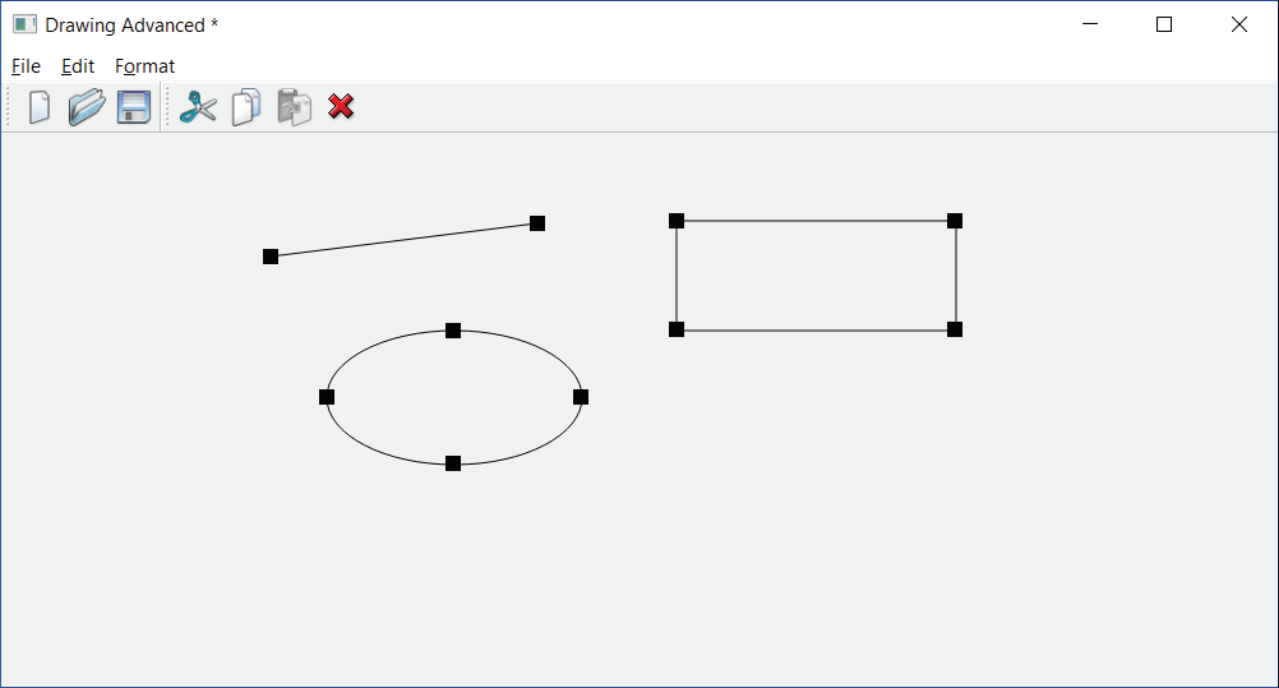
\includegraphics[width=0.9\textwidth]{images/p284_i03.png}\end{center}

\section{改进编辑器}

本章的编辑器是第 5 章「Qt 图形应用」中编辑器的更高级版本。在这一版本中，我们可以更改文本的字体和对齐方式，可以标记文本，还可以剪切粘贴文本。

\subsection{EditorWindow 类}

本章的 EditorWindow 类与第 5 章「Qt 图形应用」中的类相似。它捕获按键事件和窗口关闭事件。

\medskip\noindent{\ttfamily\bfseries EditorWindow.h}

\begin{codebox}
#ifndef EDITORWINDOW_H
#define EDITORWINDOW_H

#include <QMainWindow>
#include <QActionGroup>
#include <QPair>
#include <QMap>

#include "..\MainWindow\MainWindow.h"
#include "EditorWidget.h"

class EditorWindow : public MainWindow {
  Q_OBJECT

  public:
    EditorWindow(QWidget *parentWidgetPtr = nullptr);
    ~EditorWindow();

  protected:
    void keyPressEvent(QKeyEvent* eventPtr);
    void closeEvent(QCloseEvent* eventPtr);

  private:
    EditorWidget* m_editorWidgetPtr;
    QActionGroup* m_alignmentGroupPtr;
};

#endif // EDITORWINDOW_H
\end{codebox}

\medskip\noindent{\ttfamily\bfseries EditorWindow.cpp}

\begin{codebox}
#include "EditorWindow.h"
#include <QtWidgets>
\end{codebox}

构造函数初始化编辑器窗口。它把窗口尺寸设置为 1000×500 像素，动态创建一个编辑器部件，并添加标准的 File 和 Edit 菜单：

\begin{codebox}
EditorWindow::EditorWindow(QWidget *parentWidgetPtr /*= nullptr*/)
 :MainWindow(parentWidgetPtr) {
  resize(1000, 500);

  m_editorWidgetPtr = new EditorWidget(this);
  setCentralWidget(m_editorWidgetPtr);
  addFileMenu();
  addEditMenu();
\end{codebox}

与第 5 章「Qt 图形应用」相比，Format 菜单有所不同。我们添加 Font 菜单项和 Alignment 子菜单，再往子菜单里加入左对齐、居中、右对齐三个菜单项：

\begin{codebox}
  { QMenu* formatMenuPtr = menuBar()->addMenu(tr("F&ormat"));
    connect(formatMenuPtr, SIGNAL(aboutToShow()), this,
          SLOT(onMenuShow()));

    addAction(formatMenuPtr, tr("&Font"), SLOT(onFont()),
          0, QString(), nullptr, QString(),
          LISTENER(isFontEnabled));

    { QMenu* alignmentMenuPtr =
           formatMenuPtr->addMenu(tr("&Alignment"));
      connect(alignmentMenuPtr, SIGNAL(aboutToShow()),
            this, SLOT(onMenuShow()));
\end{codebox}

我们还为 Alignment 菜单添加一个工具栏：

\begin{codebox}
      QToolBar* alignmentToolBarPtr = addToolBar(tr("Alignment"));
      m_alignmentGroupPtr = new QActionGroup(this);

      addAction(alignmentMenuPtr, tr("&Left"), SLOT(onLeft()),
               QKeySequence(Qt::ALT + Qt::Key_L), tr("left"),
               alignmentToolBarPtr, tr("Left-aligned text"),
               nullptr, LISTENER(isLeftChecked));

      addAction(alignmentMenuPtr, tr("&Center"),
               SLOT(onCenter()),
               QKeySequence(Qt::ALT + Qt::Key_C),
               tr("center"), alignmentToolBarPtr,
               tr("Center-aligned text"), nullptr,
               LISTENER(isCenterChecked));

      addAction(alignmentMenuPtr, tr("&Right"),
               SLOT(onRight()),
               QKeySequence(Qt::ALT + Qt::Key_R),
               tr("right"), alignmentToolBarPtr,
               tr("Right-aligned text"), nullptr,
               LISTENER(isRightChecked));
    }
  }

  m_editorWidgetPtr->setModifiedFlag(false);
}

EditorWindow::~EditorWindow() {
 delete m_alignmentGroupPtr;
}
\end{codebox}

按键事件和窗口关闭事件都会传递给编辑器部件：

\begin{codebox}
void EditorWindow::keyPressEvent(QKeyEvent* eventPtr) {
  m_editorWidgetPtr->keyPressEvent(eventPtr);
}

void EditorWindow::closeEvent(QCloseEvent* eventPtr) {
  m_editorWidgetPtr->closeEvent(eventPtr);
}
\end{codebox}

\subsection{EditorWidget 类}

EditorWidget 类与第 5 章「Qt 图形应用」的版本相似，不过新增了处理字体和对齐的方法与监听器。

\medskip\noindent{\ttfamily\bfseries EditorWidget.h}

\begin{codebox}
#ifndef EDITORWIDGET_H
#define EDITORWIDGET_H

#include <QWidget>
#include <QMap>
#include <QMenu>
#include <QToolBar>
#include <QPair>
#include "Caret.h"

#include "..\MainWindow\Listener.h"
#include "..\MainWindow\DocumentWidget.h"

class EditorWidget : public DocumentWidget {
  Q_OBJECT

  public:
    EditorWidget(QWidget* parentWidgetPtr);
    void keyPressEvent(QKeyEvent* eventPtr);

    private:
    void keyEditPressEvent(QKeyEvent* eventPtr);
    void keyMarkPressEvent(QKeyEvent* eventPtr);
\end{codebox}

用户按下鼠标按钮、移动鼠标和松开鼠标按钮时会分别调用 mousePressEvent、mouseMoveEvent 和 mouseReleaseEvent：

\begin{codebox}
  public:
    void mousePressEvent(QMouseEvent* eventPtr);
    void mouseMoveEvent(QMouseEvent* eventPtr);
    void mouseReleaseEvent(QMouseEvent* eventPtr);

    private:
    int mouseToIndex(QPoint point);

    public:
    void paintEvent(QPaintEvent* eventPtr);
    void resizeEvent(QResizeEvent* eventPtr);
\end{codebox}

用户选择 New 菜单项时会调用 newDocument 方法；用户选择 Save 或 Save As 时会调用 writeFile；用户选择 Open 菜单项时会调用 readFile：

\begin{codebox}
    private:
      void newDocument(void);
      bool writeFile(const QString& filePath);
      bool readFile(const QString& filePath);

    public slots:
      bool isCopyEnabled();
      void onCopy(void);
      bool isPasteEnabled();
      void onPaste(void);
      void onDelete(void);

      DEFINE_LISTENER(EditorWidget, isFontEnabled);
      void onFont(void);
\end{codebox}

Alignment 子菜单变为可见之前会调用 isLeftChecked、isCenterChecked 和 isRightChecked 方法。它们随后给当前选中的对齐方式标注一个单选按钮：

\begin{codebox}
      DEFINE_LISTENER(EditorWidget, isLeftChecked);
      DEFINE_LISTENER(EditorWidget, isCenterChecked);
      DEFINE_LISTENER(EditorWidget, isRightChecked);
\end{codebox}

用户选择 Alignment 子菜单中的某个菜单项时会调用 onLeft、onCenter 和 onRight 方法：

\begin{codebox}
      void onLeft(void);
      void onCenter(void);
      void onRight(void);

      private:
       void setCaret();
       void simulateMouseClick(int x, int y);
\end{codebox}

在本版的编辑器中，我们有两种模式：edit（编辑）和 mark（标记）。用户输入文本或用方向键移动光标时，edit 模式处于活动状态；用户用鼠标标记了一段文本时，mark 模式处于活动状态。光标在 edit 模式下可见，在 mark 模式下不可见：

\begin{codebox}
  private:
    enum Mode {Edit, Mark} m_mode;
\end{codebox}

文本可以在左对齐、居中和右对齐三个方向上对齐：

\begin{codebox}
   enum Alignment {Left, Center, Right} m_alignment;
\end{codebox}

在 edit 模式下，\texttt{m\_editIndex} 存放下一个将由用户输入的字符要放置的索引，它同时也是光标的位置。在 mark 模式下，\texttt{m\_firstIndex} 和 \texttt{m\_lastIndex} 存放第一个和最后一个被标记字符的索引：

\begin{codebox}
    int m_editIndex, m_firstIndex, m_lastIndex;
\end{codebox}

\texttt{m\_caret} 对象持有编辑器的光标。光标在 edit 模式下可见，在 mark 模式下不可见：

\begin{codebox}
    Caret m_caret;
\end{codebox}

\texttt{m\_editorText} 字段存放编辑器的文本，\texttt{m\_copyText} 存放用户剪切或复制的文本：

\begin{codebox}
     QString m_editorText, m_copyText;
\end{codebox}

编辑器的文本按行划分；每行第一个和最后一个字符的索引存放在 \texttt{m\_lineList} 中：

\begin{codebox}
    QList<QPair<int,int>> m_lineList;
\end{codebox}

文本当前字体存放在 \texttt{m\_textFont} 中。当前字体下一个字符的高度（以像素为单位）存放在 \texttt{m\_fontHeight} 中：

\begin{codebox}
    QFont m_textFont;
    int m_fontHeight;
\end{codebox}

mousePressEvent 和 mouseMoveEvent 方法保存最近的鼠标点，以便计算鼠标事件之间的距离：

\begin{codebox}
    Qt::MouseButton m_button;
\end{codebox}

与第 5 章「Qt 图形应用」中的方法类似，calculate 是一个辅助方法，用于计算文本中每个字符的外接矩形。不过，本章的版本更复杂，因为它必须考虑文本是左对齐、居中对齐还是右对齐：

\begin{codebox}
    void calculate();
\end{codebox}

外接矩形存放在 \texttt{m\_rectList} 中，随后供光标和 paintEvent 使用：

\begin{codebox}
     QList<QRect> m_rectList;
   };

#endif // EDITORWIDGET_H
\end{codebox}

\medskip\noindent{\ttfamily\bfseries EditorWidget.cpp}

\begin{codebox}
#include "EditorWidget.h"
#include <QtWidgets>
#include <CAssert>
using namespace std;
\end{codebox}

构造函数把窗口标题设置为 Editor Advanced，把文件后缀设置为 edi：

\begin{codebox}
EditorWidget::EditorWidget(QWidget* parentWidgetPtr)
 :DocumentWidget(tr("Editor Advanced"),
     tr("Editor files (*.edi)"), parentWidgetPtr),
\end{codebox}

文本字体初始化为 12 磅的 Times New Roman。应用模式设置为 edit，下一个将由用户输入的字符的索引设置为零，文本从一开始就是左对齐的：

\begin{codebox}
      m_textFont(tr("Times New Roman"), 12),
      m_mode(Edit),
      m_editIndex(0),
      m_alignment(Left),
      m_caret(this) {
\end{codebox}

字符的外接矩形由 calculate 计算；光标被初始化并显示，因为应用从一开始就处于 edit 模式：

\begin{codebox}
  calculate();
  setCaret();
  m_caret.show();
}
\end{codebox}

用户选择 New 菜单项时会调用 newDocument 方法。我们首先把应用模式设置为 edit，把编辑索引设为零。文本字体设置为 12 磅的 Times New Roman。编辑器的文本被清空，字符的外接矩形由 calculate 计算，光标被设置：

\begin{codebox}
void EditorWidget::newDocument(void) {
  m_mode = Edit;
  m_editIndex = 0;
  m_textFont = QFont(tr("Times New Roman"), 12);
  m_editorText.clear();
  calculate();
  setCaret();
}
\end{codebox}

用户选择 Save 或 Save As 菜单项时会调用 writeFile 方法。文件格式相当简单：我们在第一行写出字体，随后几行写出编辑器的文本：

\begin{codebox}
bool EditorWidget::writeFile(const QString& filePath) {
  QFile file(filePath);
  if (file.open(QIODevice::WriteOnly | QIODevice::Text)) {
    QTextStream outStream(&file);
    outStream << m_textFont.toString() << endl << m_editorText;
\end{codebox}

我们利用输入流的 Ok 字段判断写出是否成功：

\begin{codebox}
   return ((bool) outStream.Ok);
}
\end{codebox}

如果文件未能为写出而打开，我们返回 false：

\begin{codebox}
   return false;
}
\end{codebox}

用户选择 Open 菜单项时会调用 readFile 方法。与前面的 writeFile 类似，我们先读取第一行并用它初始化文本字体，然后读取编辑器文本：

\begin{codebox}
bool EditorWidget::readFile(const QString& filePath) {
  QFile file(filePath);
  if (file.open(QIODevice::ReadOnly | QIODevice::Text)) {
    QTextStream inStream(&file);
    m_textFont.fromString(inStream.readLine());
    m_editorText = inStream.readAll();
\end{codebox}

文本读取完毕后，我们调用 calculate 来计算文本中各字符的外接矩形，然后设置光标，并返回 true——因为读取成功了：

\begin{codebox}
  calculate();
  setCaret();
\end{codebox}

我们利用输入流的 Ok 字段判断读取是否成功：

\begin{codebox}
   return ((bool) inStream.Ok);
}
\end{codebox}

如果文件未能为读取而打开，我们返回 false：

\begin{codebox}
   return false;
}
\end{codebox}

Edit 菜单变为可见之前会调用 isCopyEnabled 方法。框架也会调用它来决定复制工具栏图标是否应被启用。如果应用处于 mark 模式，它就返回 true（菜单项随即被启用）——这意味着用户已经标记了一部分文本，可以复制了：

\begin{codebox}
bool EditorWidget::isCopyEnabled() {
  return (m_mode == Mark);
}
\end{codebox}

用户选择 Copy 菜单项时会调用 onCopy 方法。我们把被标记的文本复制到 \texttt{m\_editorText} 中：

\begin{codebox}
void EditorWidget::onCopy(void) {
  int minIndex = qMin(m_firstIndex, m_lastIndex),
  maxIndex = qMax(m_firstIndex, m_lastIndex);

  m_copyText =
    m_editorText.mid(minIndex, maxIndex - minIndex + 1);
}
\end{codebox}

Edit 菜单变为可见之前也会调用 isPasteEnabled 方法。如果复制文本非空，它就返回 true（菜单项随即可见）。也就是说，只要有一块已复制、待粘贴的文本，它就返回 true：

\begin{codebox}
bool EditorWidget::isPasteEnabled() {
  return !m_copyText.isEmpty();
}
\end{codebox}

用户选择 Paste 菜单项时会调用 onPaste 方法。在 mark 模式下，我们调用 onDelete，被标记的文本随即被删除：

\begin{codebox}
void EditorWidget::onPaste(void) {
  if (m_mode == Mark) {
     onDelete();
  }
\end{codebox}

然后，我们把复制的文本插入编辑器文本。我们还更新 \texttt{m\_editIndex}，因为文本插入之后的编辑索引应位于被插入文本之后的位置：

\begin{codebox}
  m_editorText.insert(m_editIndex, m_copyText);
  m_editIndex += m_copyText.size();
\end{codebox}

最后，我们计算文本中各字符的外接矩形，把光标设置到新索引处，设置已修改标记——因为文本已被改变——并调用 update 来强制在合适时机调用 paintEvent，以显示新文本：

\begin{codebox}
  calculate();
  setCaret();
  setModifiedFlag(true);
  update();
}
\end{codebox}

用户选择 Delete 菜单项或 Delete 工具栏图标时会调用 onDelete 方法。其效果与用户按下 Delete 键的事件类似。因此，我们准备一个带 Delete 键的按键事件，把它作为参数用在 keyPressEvent 的调用中。

注意，没有 isDeleteEnabled 方法，因为用户总是可以使用 Delete 菜单项。在 edit 模式下，删除下一个字符；在 mark 模式下，删除被标记的文本：

\begin{codebox}
void EditorWidget::onDelete(void) {
  QKeyEvent event(QEvent::KeyPress, Qt::Key_Delete,
              Qt::NoModifier);
  keyPressEvent(&event);
}
\end{codebox}

Format 菜单变为可见之前会调用 isCopyEnabled。在 edit 模式下它返回 true——因为当只有一部分字符被标记时，更改所有字符的字体是不合逻辑的：

\begin{codebox}
bool EditorWidget::isFontEnabled() {
  return (m_mode == Edit);
}
\end{codebox}

用户选择 Font 菜单项时会调用 onFont 方法。我们让用户通过 Qt 的 QFontDialog 类选择新字体：

\begin{codebox}
void EditorWidget::onFont(void) {
   bool pressedOkButton;
   QFont newFont =
     QFontDialog::getFont(&pressedOkButton, m_textFont, this);
\end{codebox}

如果用户按下 Ok 按钮关闭对话框，我们就设置编辑器的字体字段（\texttt{m\_textFont}）和已修改标记：

\begin{codebox}
   if (pressedOkButton) {
     m_textFont = newFont;
     setModifiedFlag(true);
\end{codebox}

我们通过调用 calculate 计算新的外接矩形，设置光标，并调用 update 来强制在合适时机调用 paintEvent：

\begin{codebox}
     calculate();
     m_caret.set(m_rectList[m_editIndex]);
     update();
   }
}
\end{codebox}

Alignment 子菜单变为可见之前会调用 isLeftChecked、isCenterChecked 和 isRightChecked 方法。它们针对当前的对齐方式返回 true：

\begin{codebox}
bool EditorWidget::isLeftChecked(void) {
  return (m_alignment == Left);
}

bool EditorWidget::isCenterChecked(void) {
  return (m_alignment == Center);
}

bool EditorWidget::isRightChecked(void) {
  return (m_alignment == Right);
}
\end{codebox}

用户选择 Left、Center 和 Right 菜单项时会调用 onLeft、onCenter 和 onRight 方法。它们设置对齐方式和已修改标记，计算新的外接矩形，设置光标，并调用 update 来强制在合适时机调用 paintEvent：

\begin{codebox}
void EditorWidget::onLeft(void) {
  m_alignment = Left;
  setModifiedFlag(true);
  calculate();
  setCaret();
  update();
}

void EditorWidget::onCenter(void) {
  m_alignment = Center;
  setModifiedFlag(true);
  calculate();
  setCaret();
  update();
}

void EditorWidget::onRight(void) {
  m_alignment = Right;
  setModifiedFlag(true);
  calculate();
  setCaret();
  update();
}
\end{codebox}

用户按下某个鼠标按钮时会调用 mousePressEvent 方法。我们调用 mouseToIndex 来找到用户点击的字符索引。眼下，第一个和最后一个标记索引都被设置为鼠标索引。最后一个索引随后可能被下一小段中的 mouseMoveEvent 调用改变。最后，模式被设置为 mark，光标被隐藏：

\begin{codebox}
void EditorWidget::mousePressEvent(QMouseEvent* eventPtr) {
  if (eventPtr->buttons() == Qt::LeftButton) {
     m_firstIndex = m_lastIndex = mouseToIndex(eventPtr->pos());
     m_mode = Mark;
     m_caret.hide();
   }
}
\end{codebox}

用户移动鼠标时会调用 mouseMoveEvent 方法。我们把最后一个标记索引设置为鼠标索引，并调用 update 来强制在合适时机调用 paintEvent：

\begin{codebox}
void EditorWidget::mouseMoveEvent(QMouseEvent* eventPtr) {
  if (eventPtr->buttons() == Qt::LeftButton) {
     m_lastIndex = mouseToIndex(eventPtr->pos());
     update();
  }
}
\end{codebox}

用户松开鼠标按钮时会调用 mouseReleaseEvent 方法。如果用户把鼠标移回了本次鼠标移动的起始位置，就没有任何需要标记的内容，我们把应用设置为 edit 模式。此时，我们把编辑索引设置为第一个标记索引，设置并显示光标（因为在 edit 模式下光标应当可见）。最后，我们调用 update 来强制在合适时机调用 paintEvent：

\begin{codebox}
void EditorWidget::mouseReleaseEvent(QMouseEvent* eventPtr) {
  if (eventPtr->buttons() == Qt::LeftButton) {
    if (m_firstIndex == m_lastIndex) {
      m_mode = Edit;
      m_editIndex = m_firstIndex;
      setCaret();
      m_caret.show();
      update();
    }
  }
}
\end{codebox}

用户按下键盘上的某个键时会调用 keyPressEvent。根据应用模式（edit 或 mark），我们调用 keyEditPressEvent 或后面的 keyMarkPressEvent 来进一步处理按键事件：

\begin{codebox}
void EditorWidget::keyPressEvent(QKeyEvent* eventPtr) {
   switch (m_mode) {
     case Edit:
     keyEditPressEvent(eventPtr);
     break;

     case Mark:
     keyMarkPressEvent(eventPtr);
     break;
   }
}
\end{codebox}

keyEditPressEvent 处理 edit 模式下的按键。我们首先检查按键是否为方向键、上翻页键、下翻页键、Delete 键、Backspace 键或回车键：

\begin{codebox}
void EditorWidget::keyEditPressEvent(QKeyEvent* eventPtr) {
  switch (eventPtr->key()) {
\end{codebox}

对于左方向键，我们把编辑索引向后移动一步，除非它已经位于文本的开头：

\begin{codebox}
   case Qt::Key_Left:
     if (m_editIndex > 0) {
        --m_editIndex;
     }
     break;
\end{codebox}

对于右方向键，我们把编辑索引向前移动一步，除非它已经位于文本的末尾：

\begin{codebox}
   case Qt::Key_Right:
    if (m_editIndex < m_editorText.size()) {
      ++m_editIndex;
    }
    break;
\end{codebox}

对于上方向键，我们计算上一行相应字符的 x 和 y 位置，除非它已经位于文本的顶端。然后我们调用 simulateMouseClick，它的效果如同用户点击了上一行中的字符：

\begin{codebox}
   case Qt::Key_Up: {
     QRect charRect = m_rectList[m_editIndex];

     if (charRect.top() > 0) {
       int x = charRect.left() + (charRect.width() / 2),
           y = charRect.top() - 1;
       simulateMouseClick(x, y);
     }
   }
   break;
\end{codebox}

同样，对于下方向键，我们把编辑索引向下移动一行，除非它已经位于文本的底部。我们计算下一行相应字符的 x 和 y 位置，并调用 simulateMouseClick，它的效果如同用户点击了该位置的字符：

\begin{codebox}
   case Qt::Key_Down: {
     QRect charRect = m_rectList[m_editIndex];
     int x = charRect.left() + (charRect.width() / 2),
         y = charRect.bottom() + 1;
     simulateMouseClick(x, y);
   }
   break;
\end{codebox}

对于 Delete 键，我们删除当前字符，除非我们位于文本的末尾。也就是说，除非我们正好在最后一个字符之后一步的位置：

\begin{codebox}
   case Qt::Key_Delete:
    if (m_editIndex < m_editorText.size()) {
      m_editorText.remove(m_editIndex, 1);
      setModifiedFlag(true);
    }
    break;
\end{codebox}

对于退格键，我们把编辑索引向后移动一步——除非它已经位于文本的开头——然后调用 onDelete。这样，我们就删除了前一个字符，并把编辑索引向后移动了一步：

\begin{codebox}
   case Qt::Key_Backspace:
   if (m_editIndex > 0) {
     --m_editIndex;
     onDelete();
   }
   break;
\end{codebox}

对于回车键，我们简单地在文本中插入换行符：

\begin{codebox}
   case Qt::Key_Return:
     m_editorText.insert(m_editIndex++, 'n');
     setModifiedFlag(true);
     break;
\end{codebox}

如果按键不是特殊键，我们就调用按键事件指针的 text 来检查它是否为常规字符。如果文本非空，就把它的第一个字符加入文本：

\begin{codebox}
   default: {
     QString text = eventPtr->text();

     if (!text.isEmpty()) {
       m_editorText.insert(m_editIndex++, text[0]);
       setModifiedFlag(true);
     }
   }
   break;
  }
\end{codebox}

最后，我们计算外接矩形，设置光标，并调用 update 来强制在合适时机调用 paintEvent：

\begin{codebox}
  calculate();
  setCaret();
  update();
}
\end{codebox}

用户在 mark 模式下按键时会调用 keyMarkPressEvent：

\begin{codebox}
void EditorWidget::keyMarkPressEvent(QKeyEvent* eventPtr) {
  switch (eventPtr->key()) {
\end{codebox}

对于左方向键，我们把应用设置为 edit 模式，并把编辑索引设置为第一个和最后一个标记索引中的较小者。不过，如果较小索引位于文本的开头，我们就什么都不做：

\begin{codebox}
   case Qt::Key_Left: {
     int minIndex = qMin(m_firstIndex, m_lastIndex);

     if (minIndex > 0) {
       m_mode = Edit;
       m_caret.show();
       m_editIndex = minIndex;
     }
   }
   break;
\end{codebox}

反过来，对于右方向键，我们把应用设置为 edit 模式，并把编辑索引设置为第一个和最后一个标记索引中的较大者。不过，如果较大索引位于文本的末尾，我们就什么都不做：

\begin{codebox}
   case Qt::Key_Right: {
     int maxIndex = qMax(m_firstIndex, m_lastIndex);

     if (maxIndex < m_editorText.size()) {
       m_mode = Edit;
       m_caret.show();
       m_editIndex = maxIndex;
     }
   }
   break;
\end{codebox}

对于上、下方向键，我们在当前行的上一行或下一行模拟一次鼠标点击，就像前面的 edit 模式那样：

\begin{codebox}
   case Qt::Key_Up: {
     QRect charRect = m_rectList[m_editIndex];

     if (charRect.top() > 0) {
       int x = charRect.left() + (charRect.width() / 2),
           y = charRect.top() - 1;
       simulateMouseClick(x, y);
     }
   }
   break;

   case Qt::Key_Down: {
     QRect charRect = m_rectList[m_editIndex];
     int x = charRect.left() + (charRect.width() / 2),
         y = charRect.bottom() + 1;
     simulateMouseClick(x, y);
   }
   break;
\end{codebox}

在 mark 模式下，Delete 键和退格键执行同样的任务——删除被标记的文本：

\begin{codebox}
   case Qt::Key_Delete:
   case Qt::Key_Backspace: {
     int minIndex = qMin(m_firstIndex, m_lastIndex),
         maxIndex = qMax(m_firstIndex, m_lastIndex);
\end{codebox}

我们把被标记的文本从编辑文本中移除，设置已修改标记，把应用设置为 edit 模式，把编辑索引设置为第一个和最后一个标记索引中的较小者，并显示光标：

\begin{codebox}
     m_editorText.remove(minIndex, maxIndex - minIndex);
     setModifiedFlag(true);
     m_mode = Edit;
     m_editIndex = minIndex;
     m_caret.show();
   }
   break;
\end{codebox}

回车键的情况与前面 edit 模式的情况类似，不同之处在于我们先删除被标记的文本，然后给编辑器文本添加一个新行：

\begin{codebox}
   case Qt::Key_Return:
     onDelete();
     m_editorText.insert(m_editIndex++, 'n');
     setModifiedFlag(true);
     break;
\end{codebox}

如果按键不是特殊键，我们就调用按键事件指针的 text 来检查它是否为常规字符。如果文本非空，说明用户输入了一个常规字符，我们把该字符插入编辑器文本：

\begin{codebox}
   default: {
     QString text = eventPtr->text();

     if (!text.isEmpty()) {
       onDelete();
       m_editorText.insert(m_editIndex++, text[0]);
       setModifiedFlag(true);
     }
   }
   break;
  }
\end{codebox}

最后，我们计算新的字符外接矩形，设置光标，并调用 update 来强制在合适时机调用 paintEvent：

\begin{codebox}
  calculate();
  setCaret();
  update();
}
\end{codebox}

用户上下移动光标时会调用 simulateMouseClick 方法。它通过调用 mousePressEvent 和 mouseReleaseEvent，并使用事先准备好的事件对象，来模拟一次鼠标点击：

\begin{codebox}
void EditorWidget::simulateMouseClick(int x, int y) {
  QMouseEvent pressEvent(QEvent::MouseButtonPress, QPointF(x, y),
      Qt::LeftButton, Qt::NoButton, Qt::NoModifier);
  mousePressEvent(&pressEvent);
  QMouseEvent releaseEvent(QEvent::MouseButtonRelease,
                 QPointF(x, y), Qt::LeftButton,
                 Qt::NoButton, Qt::NoModifier);
  mousePressEvent(&releaseEvent);
}
\end{codebox}

setCaret 方法在 edit 模式下把光标设置到合适的大小和位置。首先，我们利用 \texttt{m\_editIndex} 找到正确字符的矩形。然后，我们创建一个宽度仅为一个像素的新矩形，以便光标看起来像一条细竖线：

\begin{codebox}
void EditorWidget::setCaret() {
  QRect charRect = m_rectList[m_editIndex];
  QRect caretRect(charRect.left(), charRect.top(),
                1, charRect.height());
  m_caret.set(caretRect);
}
\end{codebox}

mouseToIndex 方法接受一个鼠标点，返回该点所在字符的索引。与第 5 章「Qt 图形应用」的版本不同，我们需要考虑文本可能居中或右对齐的情况：

\begin{codebox}
int EditorWidget::mouseToIndex(QPoint point) {
   int x = point.x(), y = point.y();
\end{codebox}

如果鼠标点位于编辑器文本的下方，就返回最后一个字符的索引：

\begin{codebox}
   if (y > (m_fontHeight * m_lineList.size())) {
     return m_editorText.size();
   }
\end{codebox}

否则，我们首先找到鼠标点所在的行，并获取该行第一个和最后一个字符的索引：

\begin{codebox}
   else {
     int lineIndex = y / m_fontHeight;
     QPair<int,int> lineInfo = m_lineList[lineIndex];
     int firstIndex = lineInfo.first, lastIndex = lineInfo.second;
\end{codebox}

如果鼠标点位于该行第一个字符的左侧（文本居中或右对齐时可能如此），我们返回该行第一个字符的索引：

\begin{codebox}
     if (x < m_rectList[firstIndex].left()) {
       return firstIndex;
    }
\end{codebox}

反过来，如果鼠标点位于该行的右侧，我们返回该行最后一个字符下一个字符的索引：

\begin{codebox}
    else if (x >= m_rectList[lastIndex].right()) {
      return (lastIndex + 1);
    }
\end{codebox}

否则，我们遍历该行中的字符，对每个字符检查鼠标点是否位于该字符的外接矩形之内：

\begin{codebox}
    else {
      for (int charIndex = firstIndex + 1;
          charIndex <= lastIndex; ++charIndex){
        int left = m_rectList[charIndex].left();
\end{codebox}

如果鼠标点位于矩形之内，我们再检查它更靠近矩形的左边框还是右边框。如果更靠近左边框，我们返回该字符的索引；如果更靠近右边框，我们则返回下一个字符的索引：

\begin{codebox}
        if (x < left) {
          int last = m_rectList[charIndex - 1].left();
          int leftSize = x - last, rightSize = left - x;
          return (leftSize < rightSize) ? (charIndex - 1)
                                        : charIndex;
        }
      }
    }
  }
\end{codebox}

按理说程序不应走到这一步。加入 assert 宏只是调试之用：

\begin{codebox}
    assert(false);
    return 0;
  }
\end{codebox}

用户调整窗口大小时会调用 resizeEvent 方法。我们重新计算字符的外接矩形，因为窗口宽度可能发生了变化，这会使每行容纳的字符数变少或变多：

\begin{codebox}
void EditorWidget::resizeEvent(QResizeEvent* eventPtr) {
  calculate();
  DocumentWidget::resizeEvent(eventPtr);
}
\end{codebox}

calculate 方法把文本划分为若干行，并计算文本中每个字符的外接矩形。每行第一个和最后一个字符的索引存放在 \texttt{m\_lineList} 中，外接矩形存放在 \texttt{m\_rectList} 中：

\begin{codebox}
void EditorWidget::calculate() {
  m_lineList.clear();
  m_rectList.clear();
\end{codebox}

我们利用 Qt 的 QFontMetrics 类来获得编辑器字体下一个字符的高度。高度存放在 \texttt{m\_fontHeight} 中。width 方法给出窗口内容区宽度（以像素为单位）：

\begin{codebox}
  QFontMetrics metrics(m_textFont);
  m_fontHeight = metrics.height();
  QList<int> charWidthList, lineWidthList;
  int windowWidth = width();
\end{codebox}

我们首先遍历编辑器文本，把文本划分为若干行：

\begin{codebox}
  { int firstIndex = 0, lineWidth = 0;
    for (int charIndex = 0; charIndex < m_editorText.size();
       ++charIndex) {
      QChar c = m_editorText[charIndex];
\end{codebox}

遇到换行符时，我们把当前行的第一个和最后一个索引加入 \texttt{m\_lineList}：

\begin{codebox}
      if (c == 'n') {
        charWidthList.push_back(1);
        lineWidthList.push_back(lineWidth);
        m_lineList.push_back
                   (QPair<int,int>(firstIndex, charIndex));
        firstIndex = charIndex + 1;
        lineWidth = 0;
      }
\end{codebox}

否则，我们调用 Qt QMetrics 对象的 width 方法来获得该字符的宽度（以像素为单位）：

\begin{codebox}
      else {
        int charWidth = metrics.width(c);
        charWidthList.push_back(charWidth);
\end{codebox}

如果该字符会使行宽超过窗口内容区宽度，我们就把第一个和最后一个索引加入 \texttt{m\_lineList}，并另起一行。

不过，有两种情况需要考虑。如果当前字符是本行的第一个字符，就出现了该字符宽度超过窗口内容区宽度的情况（虽然不大可能）。此时，我们把该字符的索引同时作为第一行和最后一个索引加入 \texttt{m\_lineList}。下一行的第一个索引就是该字符的下一个字符：

\begin{codebox}
    if ((lineWidth + charWidth) > windowWidth) {
       if (firstIndex == charIndex) {
         lineWidthList.push_back(windowWidth);
         m_lineList.push_back
              (QPair<int,int>(firstIndex, charIndex));
         firstIndex = charIndex + 1;
       }
\end{codebox}

如果当前字符不是本行的第一个字符，我们就把第一个字符和当前字符前一个字符的索引加入 \texttt{m\_lineList}。下一行的索引就变成当前字符的索引：

\begin{codebox}
       else {
          lineWidthList.push_back(lineWidth);
          m_lineList.push_back(QPair<int,int>(firstIndex,
              charIndex - 1));
          firstIndex = charIndex;
       }
       lineWidth = 0;
    }
\end{codebox}

如果该字符没有使行宽超过窗口内容区宽度，我们就简单地把该字符的宽度加到行宽上：

\begin{codebox}
    else {
      lineWidth += charWidth;
    }
    }
  }
\end{codebox}

最后，我们需要把最后一行加入 \texttt{m\_lineList}：

\begin{codebox}
    m_lineList.push_back(QPair<int,int>(firstIndex,
         m_editorText.size() - 1));
    lineWidthList.push_back(lineWidth);
  }
\end{codebox}

把文本划分为若干行之后，我们继续计算各个字符的外接矩形。我们先把 top 设为零，因为它存放的是行的顶部位置。每处理一行，它就增加一个行高：

\begin{codebox}
  { int top = 0, left;
    for (int lineIndex = 0; lineIndex < m_lineList.size();
       ++lineIndex) {
      QPair<int,int> lineInfo = m_lineList[lineIndex];
      int lineWidth = lineWidthList[lineIndex];
      int firstIndex = lineInfo.first,
         lastIndex = lineInfo.second;
\end{codebox}

根据文本的对齐方式，我们需要决定行从哪里开始。左对齐的情况下，我们把行的左端位置设为零：

\begin{codebox}
      switch (m_alignment) {
        case Left:
          left = 0;
          break;
\end{codebox}

居中对齐的情况下，我们把左端位置设为窗口内容区宽度与行宽之差的一半。这样，该行就会出现在窗口的中央：

\begin{codebox}
        case Center:
          left = (windowWidth - lineWidth) / 2;
          break;
\end{codebox}

右对齐的情况下，我们把左端位置设为窗口内容区宽度与行宽之差。这样，该行就会出现在窗口的右侧：

\begin{codebox}
        case Right:
          left = windowWidth - lineWidth;
          break;
      }
\end{codebox}

确定了行的起始左端位置以及文本中每个字符的宽度之后，我们遍历该行，计算每个字符的外接矩形：

\begin{codebox}
     for (int charIndex = firstIndex;
         charIndex <= lastIndex;++charIndex){
      int charWidth = charWidthList[charIndex];
      QRect charRect(left, top, charWidth, m_fontHeight);
      m_rectList.push_back(charRect);
      left += charWidth;
     }
\end{codebox}

对于文本的最后一行，我们还要添加一个存放最后一个字符之后位置的矩形：

\begin{codebox}
      if (lastIndex == (m_editorText.size() - 1)) {
        QRect lastRect(left, top, 1, m_fontHeight);
        m_rectList.push_back(lastRect);
      }
\end{codebox}

每处理一个新行，top 字段就增加一个行高：

\begin{codebox}
        top += m_fontHeight;
      }
    }
  }
\end{codebox}

每当窗口需要重绘时框架就会调用 paintEvent 方法，或者我们通过调用 update 强制重绘时它也会被调用。在调用 paintEvent 之前，框架会先清空窗口内容。

我们首先创建一个随后用来书写的 QPainter 对象，并设置一些渲染提示和文本字体：

\begin{codebox}
void EditorWidget::paintEvent(QPaintEvent* /* eventPtr */) {
   QPainter painter(this);
   painter.setRenderHint(QPainter::Antialiasing);
   painter.setRenderHint(QPainter::TextAntialiasing);
   painter.setFont(m_textFont);
\end{codebox}

我们计算被标记文本的最小和最大索引（尽管我们还没确定应用是否处于 mark 模式）：

\begin{codebox}
   int minIndex = qMin(m_firstIndex, m_lastIndex),
   maxIndex = qMax(m_firstIndex, m_lastIndex);
\end{codebox}

我们遍历编辑器的文本，写出每个字符，换行符除外：

\begin{codebox}
   for (int index = 0; index < m_editorText.length(); ++index) {
     QChar c = m_editorText[index];
\end{codebox}

如果字符被标记，我们就以白字黑底写出它：

\begin{codebox}
    if (c != 'n') {
      if ((m_mode == Mark) &&
          (index >= minIndex) && (index < maxIndex)) {
        painter.setPen(Qt::white);
        painter.setBackground(Qt::black);
      }
\end{codebox}

如果字符未被标记，我们就以黑字白底写出它：

\begin{codebox}
      else {
        painter.setPen(Qt::black);
        painter.setBrush(Qt::white);
      }
\end{codebox}

文本和背景的颜色都设置好之后，我们查找该字符的外接矩形，写出字符本身：

\begin{codebox}
      QRect rect = m_rectList[index];
      painter.drawText(rect, c);
    }
  }
\end{codebox}

最后，我们还绘制光标：

\begin{codebox}
    m_caret.paint(&painter);
  }
\end{codebox}

\subsection{main 函数}

main 函数与前面各应用的 main 函数相似：它创建应用，显示编辑器窗口，然后开始执行应用。

\medskip\noindent{\ttfamily\bfseries Main.cpp}

\begin{codebox}
#include "EditorWindow.h"
#include <QApplication>

int main(int argc, char *argv[]) {
  QApplication application(argc, argv);
  EditorWindow editorWindow;
  editorWindow.show();
  return application.exec();
}
\end{codebox}

程序的输出如下面的截图所示：

\begin{center}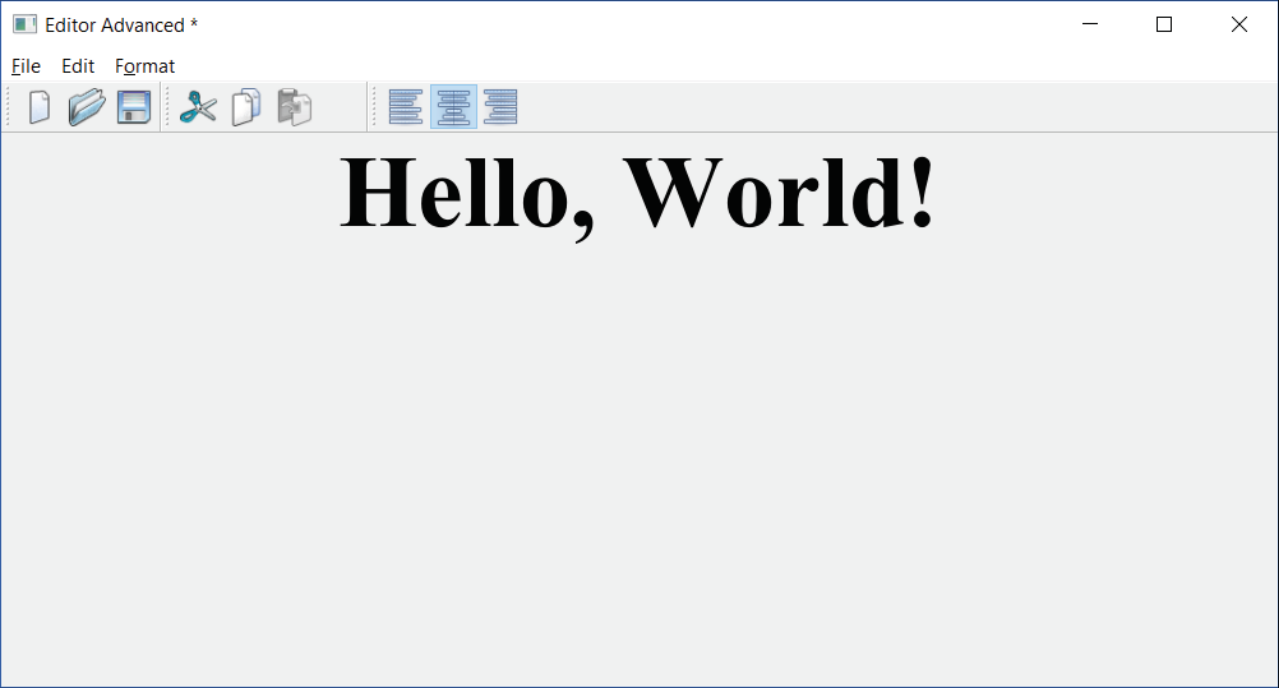
\includegraphics[width=0.9\textwidth]{images/p309_i03.png}\end{center}

\section{小结}

本章我们开发了更高级版本的模拟时钟、画图程序和编辑器。时钟显示当前的时、分、秒；画图程序允许用户绘制直线、矩形和椭圆；编辑器允许用户输入和编辑文本。钟面用数字替代了刻度线；画图程序中我们可以标记、修改和剪切粘贴图形；编辑器中我们可以更改字体和对齐方式，并标记文本块。

第 7 章将开始开发游戏奥赛罗（Othello）和圈叉棋（井字棋）。
